% !TeX program = pdflatex
\documentclass[10pt,aspectratio=169]{beamer}

% ---------------------------------------
% Langue & encodage
% ---------------------------------------
\usepackage[utf8]{inputenc}
\usepackage[T1]{fontenc}
\usepackage[french]{babel}
\usepackage{lmodern}
\usepackage{makecell}
\usepackage[absolute,overlay]{textpos}
\setlength{\TPHorizModule}{1pt}
\setlength{\TPVertModule}{1pt}

% ---------------------------------------
% Maths & utiles
% ---------------------------------------
\usepackage{amsmath, amssymb, mathtools}
\usepackage{physics}
\usepackage{siunitx}
\usepackage{graphicx}
\usepackage{booktabs}
\usepackage{tikz}
\usetikzlibrary{overlay-beamer-styles}
\usetikzlibrary{arrows.meta,positioning}
\usepackage{hyperref}

% ---------------------------------------
% Couleurs & thème minimal
% ---------------------------------------
\definecolor{Primary}{HTML}{6C5CE7}   % mauve-bleuté
\definecolor{Secondary}{HTML}{A39BFF} % plus clair
\definecolor{Accent}{HTML}{2D9CDB}    % bleu accent discret
\definecolor{Dark}{HTML}{1F2430}
\definecolor{Light}{HTML}{F6F7FB}

\setbeamercolor{normal text}{fg=Dark,bg=white}
\setbeamercolor{structure}{fg=Primary}
\setbeamercolor{title}{fg=white,bg=Primary}
\setbeamercolor{frametitle}{fg=Primary,bg=Light}
\setbeamercolor{block title}{fg=white,bg=Primary}
\setbeamercolor{block body}{bg=Light}
\setbeamercolor{itemize item}{fg=Primary}
\setbeamercolor{itemize subitem}{fg=Secondary}
\setbeamercolor{page number in head/foot}{fg=Primary}

\setbeamertemplate{navigation symbols}{} % pas d'icônes
\setbeamertemplate{frametitle}{
  \vspace{2pt}
  \begin{beamercolorbox}[wd=\paperwidth,sep=5pt,leftskip=10pt]{frametitle}
    \usebeamerfont{frametitle}\insertframetitle
    \ifx\insertframesubtitle\@empty\relax\else\\[-2pt]
      \usebeamerfont{framesubtitle}\footnotesize\insertframesubtitle
    \fi
  \end{beamercolorbox}
}

% Pied de page minimal avec numérotation
\setbeamertemplate{footline}{
  \leavevmode
  \hbox{\hspace*{\dimexpr\paperwidth-1.8cm\relax}
    \begin{beamercolorbox}[wd=1.6cm,ht=2.8ex,dp=1ex,center]{page number in head/foot}
      \insertframenumber/\inserttotalframenumber
    \end{beamercolorbox}}
  \vspace{0.2ex}
}

% Plan en début de section
\AtBeginSection[]{
  \begin{frame}{Plan}
    \tableofcontents[currentsection]
  \end{frame}
}

% ---------------------------------------
% Métadonnées
% ---------------------------------------
\title[ PFE — ENSTA Paris ]{Stratégies modernes pour l'intégration des équations d'advection-réaction-diffusion\\
{\small (ImEx \& Multi\-Résolution Adaptative)}}
\author[Alexandre EDELINE]{\textbf{Alexandre EDELINE}}
\institute[ENSTA Paris \& CMAP]{
  ENSTA Paris \\
  Laboratoire: CMAP \\
  Tuteurs laboratoire: Marc MASSOT, Christian TENAUD \\
  Tuteur ENSTA: Patrick CIARLET
}
\date{Avril - Octobre 2025}

% Optionnel : logos (placez vos fichiers dans figs/)
\titlegraphic{%
  \vspace{-2cm}
  
\includegraphics[height=3cm]{../media/0_cover/Logo_ENSTA_Paris.jpg}
  \hfill
  
\includegraphics[height=3cm]{../media/0_cover/cmap.jpg}
}

% ---------------------------------------
% Corps
% ---------------------------------------
\begin{document}

% Page de titre
{
\setbeamertemplate{footline}{} % pas de numérotation sur la page de titre
\begin{frame}[plain]
  \titlepage
\end{frame}
}

% Plan global
\begin{frame}{Plan}
  \tableofcontents
\end{frame}

% ---------------------------------------
% Slides importées (une diapo par fichier)
% ---------------------------------------
% \section{Introduction}
% Ce préambule mathématique présente divers concepts innervant dans les travaux du stage (chapitre \ref{par:contrib}). Le lecteur habitué peut ignorer ce chapitre et 
le consulter ponctuellement au besoin. Les sujets suivants y sont introduits:
\begin{enumerate}
    \item
    \item
    \item
    \item
    \item
\end{enumerate}
\section{Les équations d'advection-diffusion-réaction (ADR)}
  % \begin{frame}{Équations d'ADR}{Applications Physiques}
\end{frame}
  \begin{frame}{Applications Physiques}{Equations d'ADR}
\begin{center}
    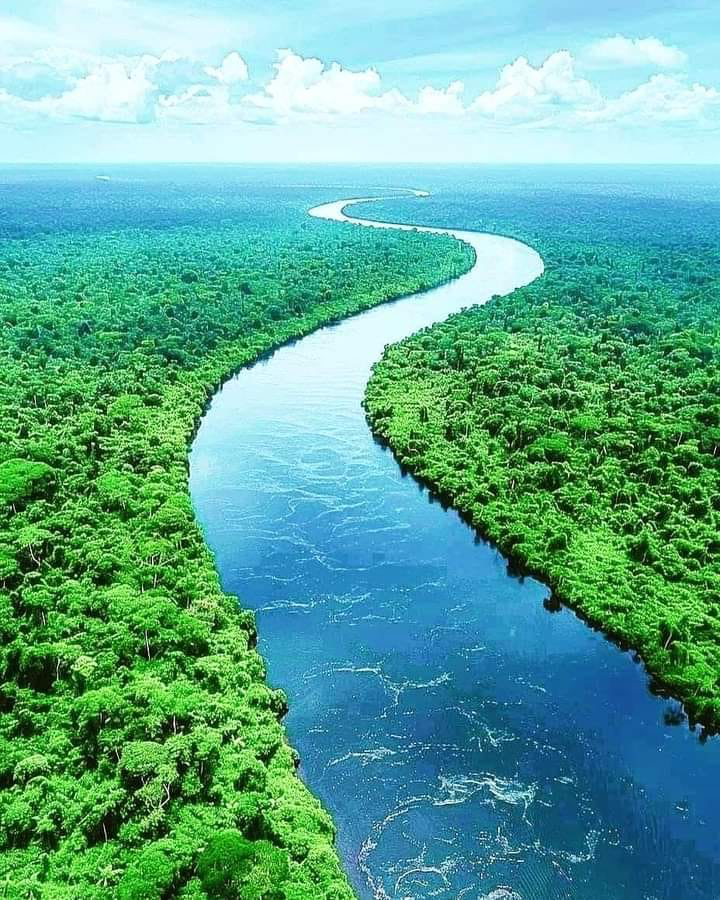
\includegraphics[height=0.4\textheight]{medias/1_/rio_amazonas.png}\hfill
    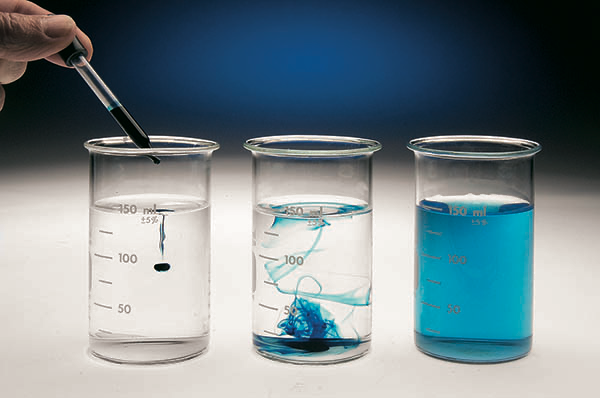
\includegraphics[height=0.4\textheight]{medias/1_/ink_diffusion.png}\hfill
    
\includegraphics[height=0.4\textheight]{medias/1_/chemical_reaction.png}
\end{center}
\pause
    \begin{equation}
        \begin{cases}
            \partial_t u(x,t) = 
                \overbrace{\underbrace{A u}_{c \partial_x u}}^{\text{Advection}}+ 
                \overbrace{\underbrace{D u}_{\partial_x(\eta \partial_x u)}}^{\text{Diffusion}}+ 
                \overbrace{\underbrace{R(u)}_{\text{Non-lin.}}}^{\text{Réaction}},\\[4pt]
            u(x,0)=u_0.
        \end{cases}
    \end{equation}

\end{frame}
  \begin{frame}{Difficultés intrinsèques}{Équations d'ADR}
% \begin{columns}[c,onlytextwidth]

    % ---- Colonne 1 : Opérateurs ----
    % \column{0.67\textwidth}
    \noindent\color{Primary}\rule{\linewidth}{0.6pt}\color{black}\\
    % ---- Colonne 2 : Multi-échelle ----
    % \column{0.30\textwidth}
    \textbf{Des solutions multi-échelles}\\[0.5em]
    \begin{itemize}
        \item plusieurs échelles de temps :\\
        \begin{itemize}
            \item chimie complexe $\tau \sim 50\mathrm{ns}$,\\
            \item advection $\mathrm{Mach }2$ sur $50\mathrm{cm}$ : $\tau \sim 10\mathrm{ms}$.
        \end{itemize}
        \item plusieurs échelles d'espace
    \end{itemize}\pause
    \noindent\color{Primary}\rule{\linewidth}{0.6pt}\color{black}\\
    \textbf{L'intégration conjointe des opérateurs}\\[0.5em]
    Les trois opérateurs ont des propriétés très différentes :
    \begin{itemize}
        \item Advection : Peu raide, raisonnant (spectre autour de $i\mathbb R$).
        \item Diffusion : Moyennement raide, spectre autour de $\mathbb R^-$.
        \item Réaction :  Très raide, hautement non-linéaire, local.
    \end{itemize}
    $\implies$ les approches monolithiques peinent.
\end{frame}

  \begin{frame}{Équations d'ADR}{Stratégies de simulation}
    \textbf{Stratégie $n^o1$ : Différencier le traitement sur chaque opérateurs}\\
        Ne pas faire un schéma monolithique.
        \begin{itemize}
            \item Séparation d'opérateurs (\emph{splitting})
            \item Méthodes ImEx (Additive Runge et Kutta)
        \end{itemize}
        \pause
\noindent\color{Primary}\rule{\linewidth}{0.6pt}\color{black}

    \textbf{Stratégie $n^o2$ : Adaptation en espace}\\
        La multirésolution adaptative : 
        \begin{itemize}
            \item Des grilles de \emph{résolution multiples},
            \item Deux opérateurs de \emph{projection/reconstruction},
            \item Représentation de la solution comme une suite de \emph{détails},
            \item Une stratégie d'\emph{adaptation}.
        \end{itemize}
    \color{red}\begin{figure}[htbp]
    \centering
\begin{tikzpicture}


\node[anchor=west] at (-6.5, -.25) {Niveau $j+1$};
\node[anchor=west] at (-6.5, .25) {Niveau $j$};
\node[anchor=west] at (-6.5, .75) {Niveau $j-1$};
% Niveau j-1

\draw (-4,.5) rectangle (0,1);
\draw (0,.5) rectangle (4,1);

    % Niveau j
\draw (-4,0) rectangle (-2,.5);
\draw (-2,0) rectangle (0,.5);
\draw (0,0) rectangle (2,.5);
\draw (2,0) rectangle (4,.5);
%\node at (1,1.75) {$k=2$};

% Niveau j+1

\draw (-4,-.5) rectangle (-3,0);
\draw (-3,-.5) rectangle (-2,0);
\draw (-2,-.5) rectangle (-1,0);
\draw (-1,-.5) rectangle (0,0);
\draw (0,-.5) rectangle (1,0);
\draw (1,-.5) rectangle (2,0);
\draw (2,-.5) rectangle (3,0);
\draw (3,-.5) rectangle (4,0);

% Relations
\node at (-2, .75) {$k=0$};
\node at (+2, .75) {$k=1$};

\node at (-3, .25) {$k=0$};
\node at (-1, .25) {$k=1$};
\node at (+1, .25) {$k=2$};
\node at (+3, .25) {$k=3$};

\node at (-3.5, -.25) {$k=0$};
\node at (-2.5, -.25) {$k=1$};
\node at (-1.5, -.25) {$k=2$};
\node at (-0.5, -.25) {$k=3$};

\node at (+0.5, -.25) {$k=4$};
\node at (+1.5, -.25) {$k=5$};
\node at (+2.5, -.25) {$k=6$};
\node at (+3.5, -.25) {$k=7$};


\end{tikzpicture}
\caption{Exemple de grille dyadique}
\label{fig:schema_sdyadique}
\end{figure}
\end{frame}
\section{Problématique}
\begin{frame}{Problématique}
\end{frame}
\begin{frame}{Présentation des contributions}
    \noindent\color{Primary}\rule{\linewidth}{0.6pt}\color{black}\\
    \textbf{Contribution $n^o1$:\\}
    \noindent\color{Primary}\rule{\linewidth}{0.6pt}\color{black}\\
    \textbf{Contribution $n^o2$:\\}
    \noindent\color{Primary}\rule{\linewidth}{0.6pt}\color{black}\\
    \textbf{Contribution $n^o3$:\\}
\end{frame}
\section{$1^{\text{ère}}$ contribution}
  Ce préambule mathématique présente divers concepts innervant dans les travaux du stage (chapitre \ref{par:contrib}). Le lecteur habitué peut ignorer ce chapitre et 
le consulter ponctuellement au besoin. Les sujets suivants y sont introduits:
\begin{enumerate}
    \item
    \item
    \item
    \item
    \item
\end{enumerate}
  \begin{frame}{Comparaison ImEx - Splitting | Nagumo}
\end{frame}
  \begin{frame}{Présentation des méthodes}{Contribution 1 | Comparaison ImEx - Splitting}

\noindent\color{Primary}\rule{\linewidth}{0.6pt}\color{black}\\
\textbf{Méthode ImEx232:\\}
Schéma à trois étages explicites et deux étages implicites, avec $\gamma = \tfrac{2-\sqrt{2}}{2}$ et $\delta = -\tfrac{2\sqrt{2}}{3}$ :
\[
\text{Explicite:}\;\begin{array}{c|ccc}
                        0 & 0 & 0 & 0\\
                        \gamma & \gamma & 0 & 0\\
                        1 & \delta & 1-\delta & 0\\ \hline
                        & 0 & 1-\gamma & \gamma
                    \end{array} \quad
\text{Implicite:}\;
                    \begin{array}{c|cc}
                        \gamma & \gamma & 0\\
                        1 & 1-\gamma & \gamma\\ \hline
                        & 1-\gamma & \gamma
                    \end{array}
\]
\pause
\noindent\color{Primary}\rule{\linewidth}{0.6pt}\color{black}\\
\textbf{Méthode ImEx222:\\}
Schéma à deux étages explicites et deux étages implicites, avec $\gamma = \tfrac{2-\sqrt{2}}{2}$ et $\delta = 1 - \tfrac{1}{2\gamma}$ :
\[
\text{Explicite:}\;
\begin{array}{c|ccc}
0 & 0 & 0 & 0\\
\gamma & \gamma & 0 & 0\\
1 & 1-\delta & \delta & 0\\ \hline
 & 1-\delta & \delta & 0
\end{array}
\quad
\text{Implicite:}\;
\begin{array}{c|cc}
\gamma & \gamma & 0\\
1 & 1-\gamma & \gamma\\ \hline
 & 1-\gamma & \gamma
\end{array}
\]
\pause
\noindent\color{Primary}\rule{\linewidth}{0.6pt}\color{black}\\
\textbf{Méthode Splitting:\\}
Splitting de Strang | Réaction : ERK2 (Heun) | Diffusion : SDIRK2 (celle des méthode ImEx).
\end{frame}

  \begin{frame}{Présentation des méthodes}{Contribution 1 | Comparaison ImEx - Splitting}

\noindent\color{Primary}\rule{\linewidth}{0.6pt}\color{black}\\
\textbf{Méthode ImEx232:\\}\tiny
Schéma à trois étages explicites et deux étages implicites, avec $\gamma = \tfrac{2-\sqrt{2}}{2}$ et $\delta = -\tfrac{2\sqrt{2}}{3}$ :
\begin{align}
\text{Explicite:}\;\begin{array}{c|ccc}
                        0 & 0 & 0 & 0\\
                        \gamma & \gamma & 0 & 0\\
                        1 & \delta & 1-\delta & 0\\ \hline
                        & 0 & 1-\gamma & \gamma
                    \end{array} \quad
\text{Implicite:}\;
                    \begin{array}{c|cc}
                        \gamma & \gamma & 0\\
                        1 & 1-\gamma & \gamma\\ \hline
                        & 1-\gamma & \gamma
                    \end{array}\; 
&\text{\textbf{équation cible générique : }} \partial_t u = f_E(u) + f_I(u) \mid \text{\textbf{objectif : }} u^n \rightarrow u^{n+1}.
\end{align}
\vspace{-2em}
\pause
\normalsize
\noindent\color{Primary}\rule{\linewidth}{0.6pt}\color{black}\\
\textbf{Calcul:}\tiny\pause
\vspace{-2em}
\begin{columns}[T]
\begin{column}{0.48 \textwidth}

\begin{align}\notag
    \uncover<2->{&\text{\color{red}\rule{2cm}{0.4pt} Initialisation \rule{2cm}{0.4pt}}\\\notag
        &u_0 = u^n,\\\notag}
    \uncover<3->{&\text{\color{red}\rule{2cm}{0.4pt} $1^{er}$ étage \rule{2cm}{0.4pt}}\\\notag
&k_1^E = f_E(u_0),k_1^I = f_I(u_1).\\\notag}
    \uncover<4->{&u_1 = u_0 + \gamma \Delta t k_1^E + \gamma \Delta t\overbrace{f_I(u_1)}^{=k^I_1},\\\notag}
        \uncover<5->{&\quad \implies u_1 = \left[Id - \gamma \Delta t f_I(\cdot)\right]^{-1}(u_0 + \gamma \Delta t k_1^E ),\\\notag}
        \uncover<6->{&\quad \implies k_1^I = f_I(u_1).}
\end{align}
\end{column}

\begin{column}{0.48 \textwidth}
\begin{align}\notag
    \uncover<7->{&\text{\color{red}\rule{2cm}{0.4pt} $2^{eme}$ étage \rule{2cm}{0.4pt}}\\\notag
    &k_2^E = f_E(u_1),k_2^I = f_I(u_2).\\\notag}
    \uncover<8->{&u_2 = u_0 + \delta \Delta t k_1^E +  (1-\delta) \Delta t k_2^E + (1-\gamma) \Delta t k^I_1 +  \overbrace{\gamma \Delta t f_I(u_2)}^{=k^I_2},\\\notag
        &\quad \implies u_1 = \left[Id - \gamma \Delta t f_I(\cdot)\right]^{-1} \left( u_0 + \delta \Delta t k_1^E +  (1-\delta) \Delta t k_2^E + (1-\gamma) \Delta t k^I_1 \right),\\\notag
        &\quad \implies k_2^I = f_I(u_2).\\\notag}
    \uncover<9->{&\text{\color{red}\rule{2cm}{0.4pt} $3^{eme}$ étage \rule{2cm}{0.4pt}}\\\notag
    &k_3^E = f_E(u2).\\\notag}
    \uncover<10->{&\text{\color{red}\rule{2cm}{0.4pt} Recombinaison des etages \rule{1cm}{0.4pt}}\\\notag
    &u^{n+1} = u^n + \Delta t \left( (1-\gamma) k^E_2 + \gamma k^E_3 + (1-\gamma) k^I_1 + \gamma k^I_2 \right).}
\end{align}
\end{column}
\end{columns}
\end{frame}

    \begin{frame}{Analyse de stabilité}{Annexe}
    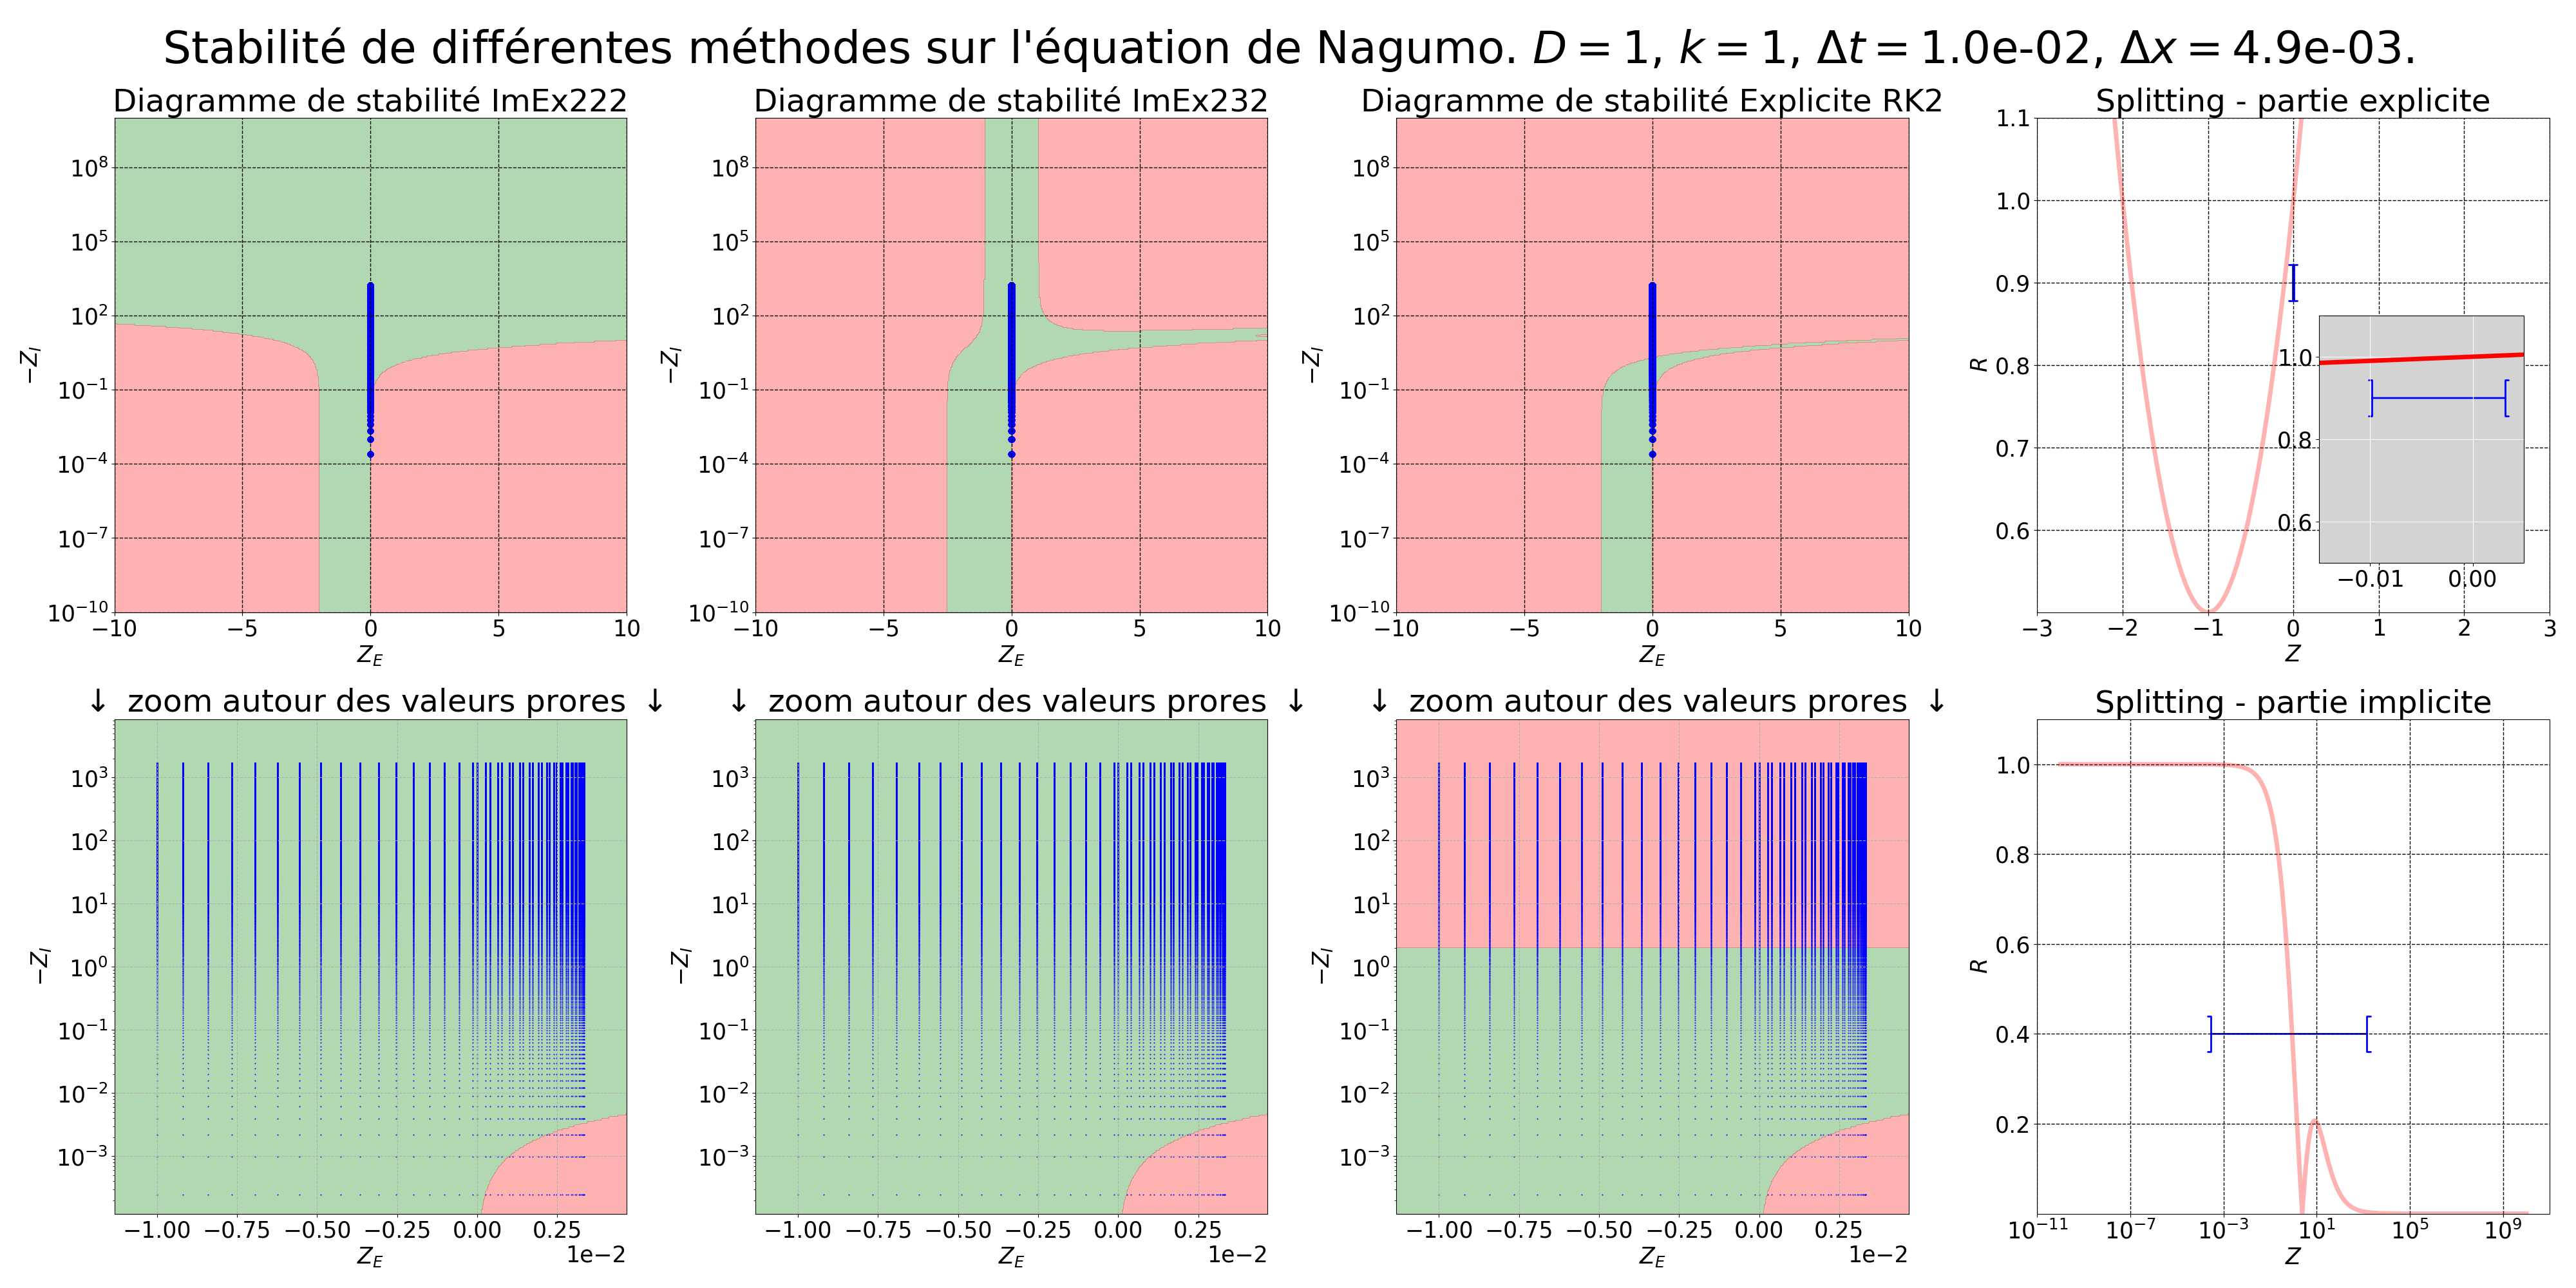
\includegraphics[width = \textwidth]{medias/2_/1_/STABILITE_D1_k1_dt1.0e-02_dx4.9e-03.png}
\end{frame}
    \begin{frame}{Contribution 1 | Comparaison ImEx - Splitting}{Analyse de stabilité}
    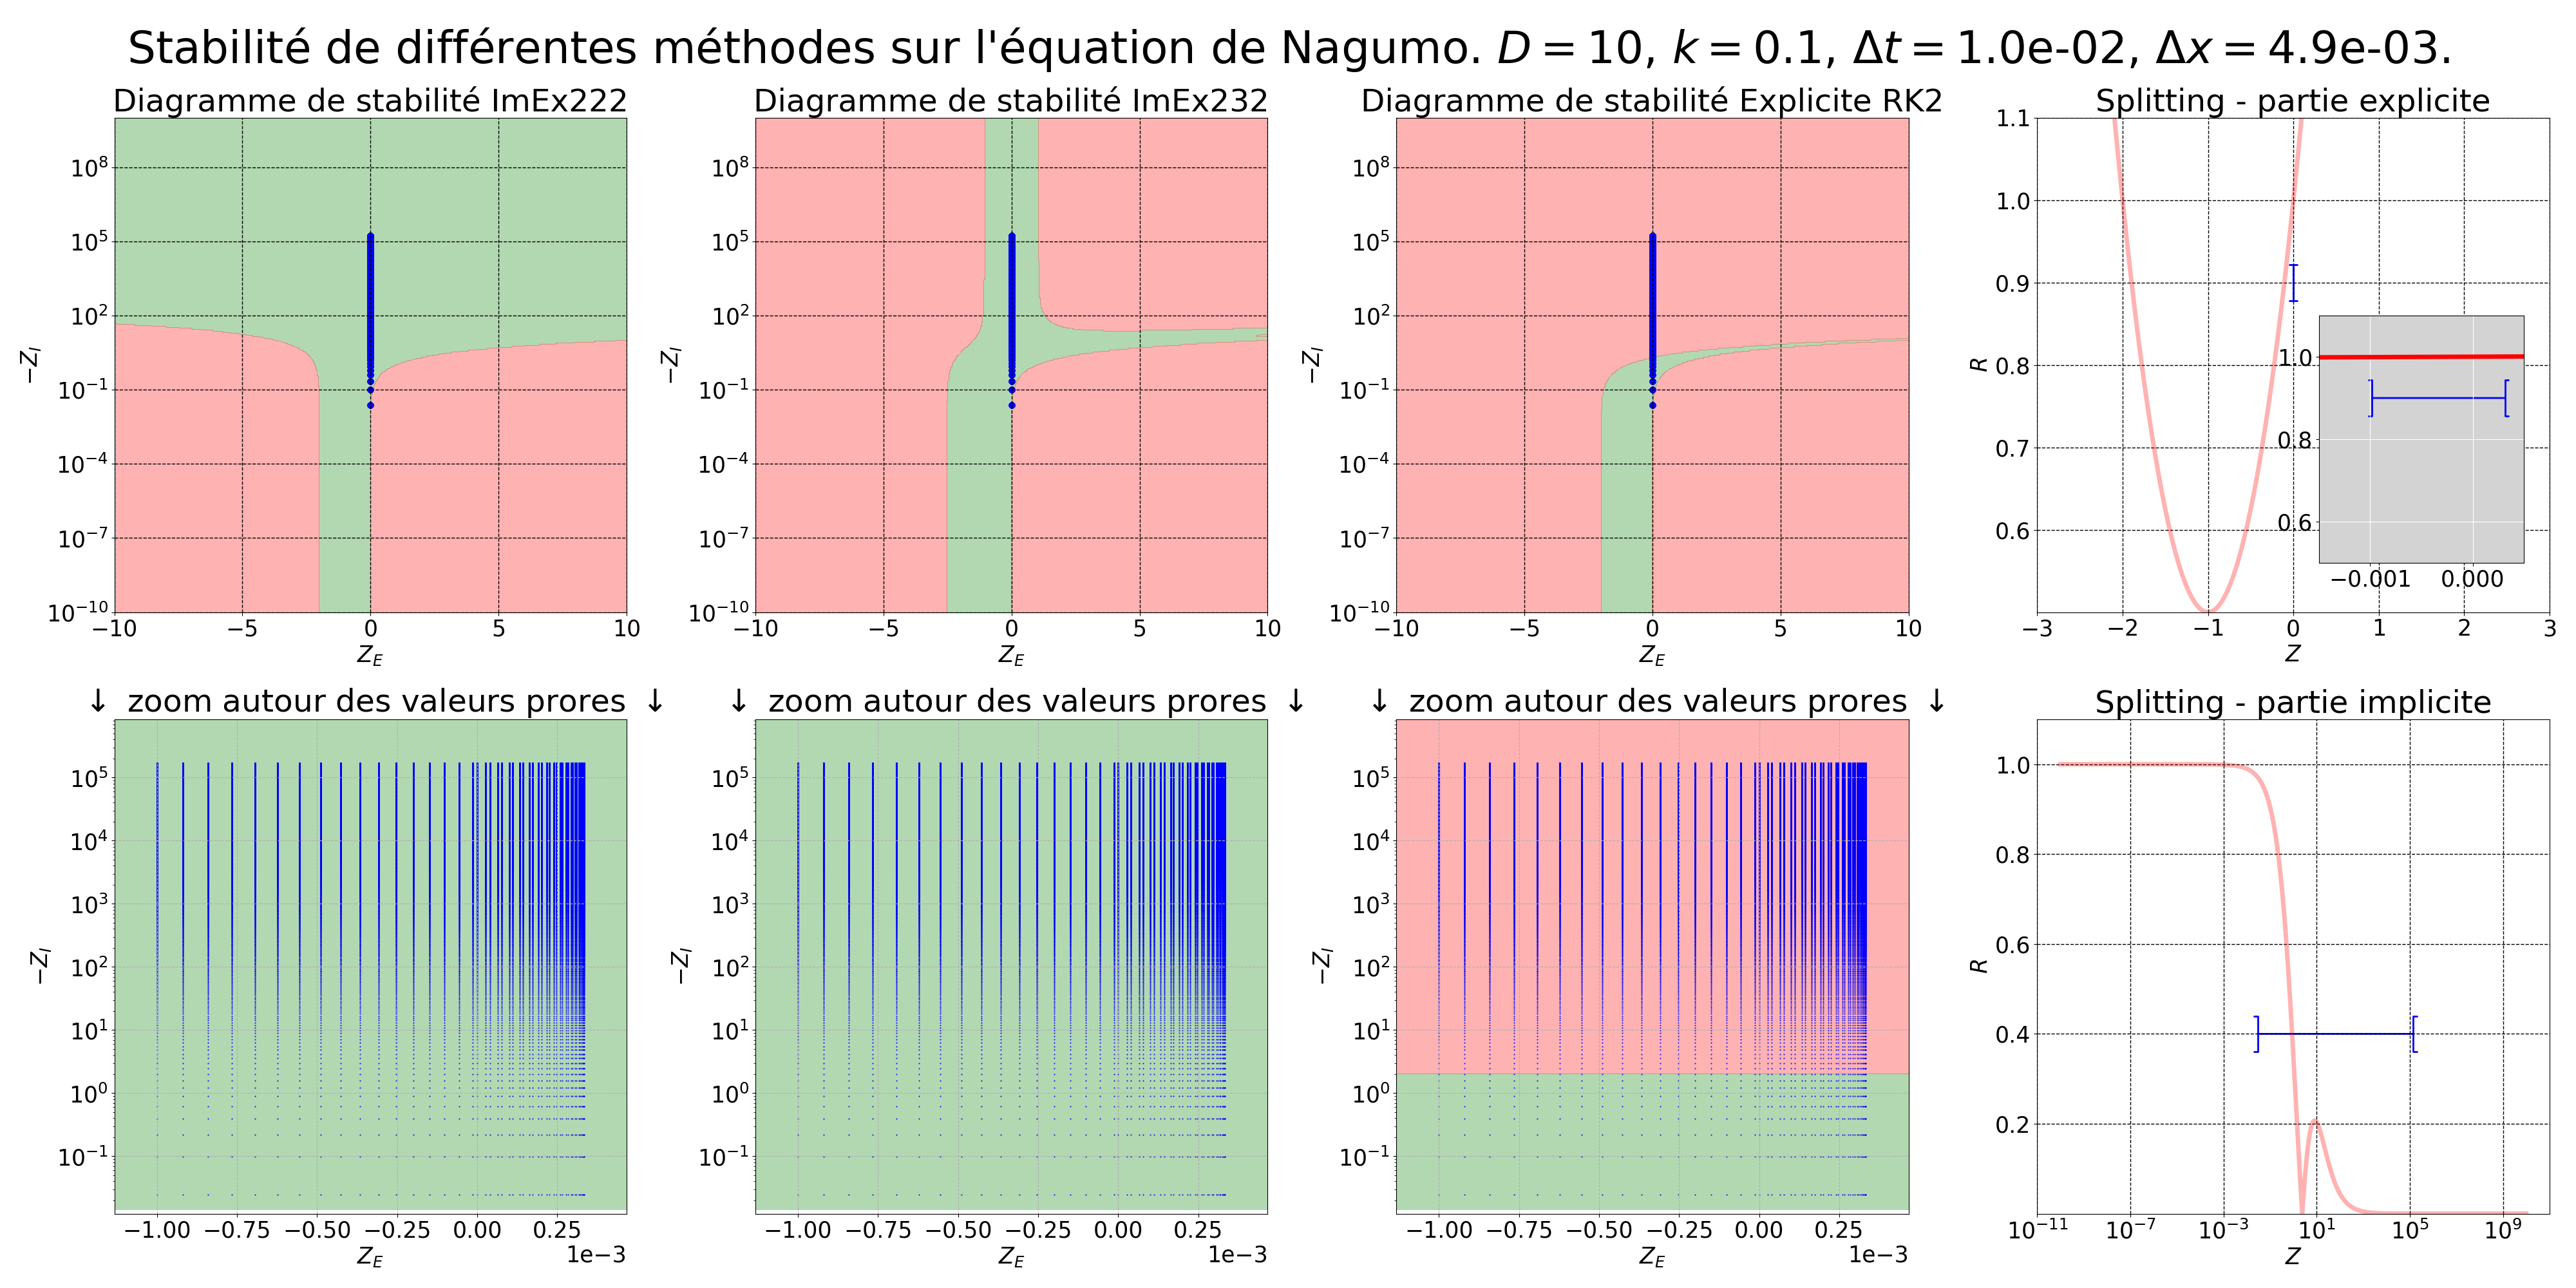
\includegraphics[width = \textwidth]{medias/2_/1_/STABILITE_D10_k0.1_dt1.0e-02_dx4.9e-03.png}
\end{frame}
    \begin{frame}{Analyse de stabilité}{Annexe}
    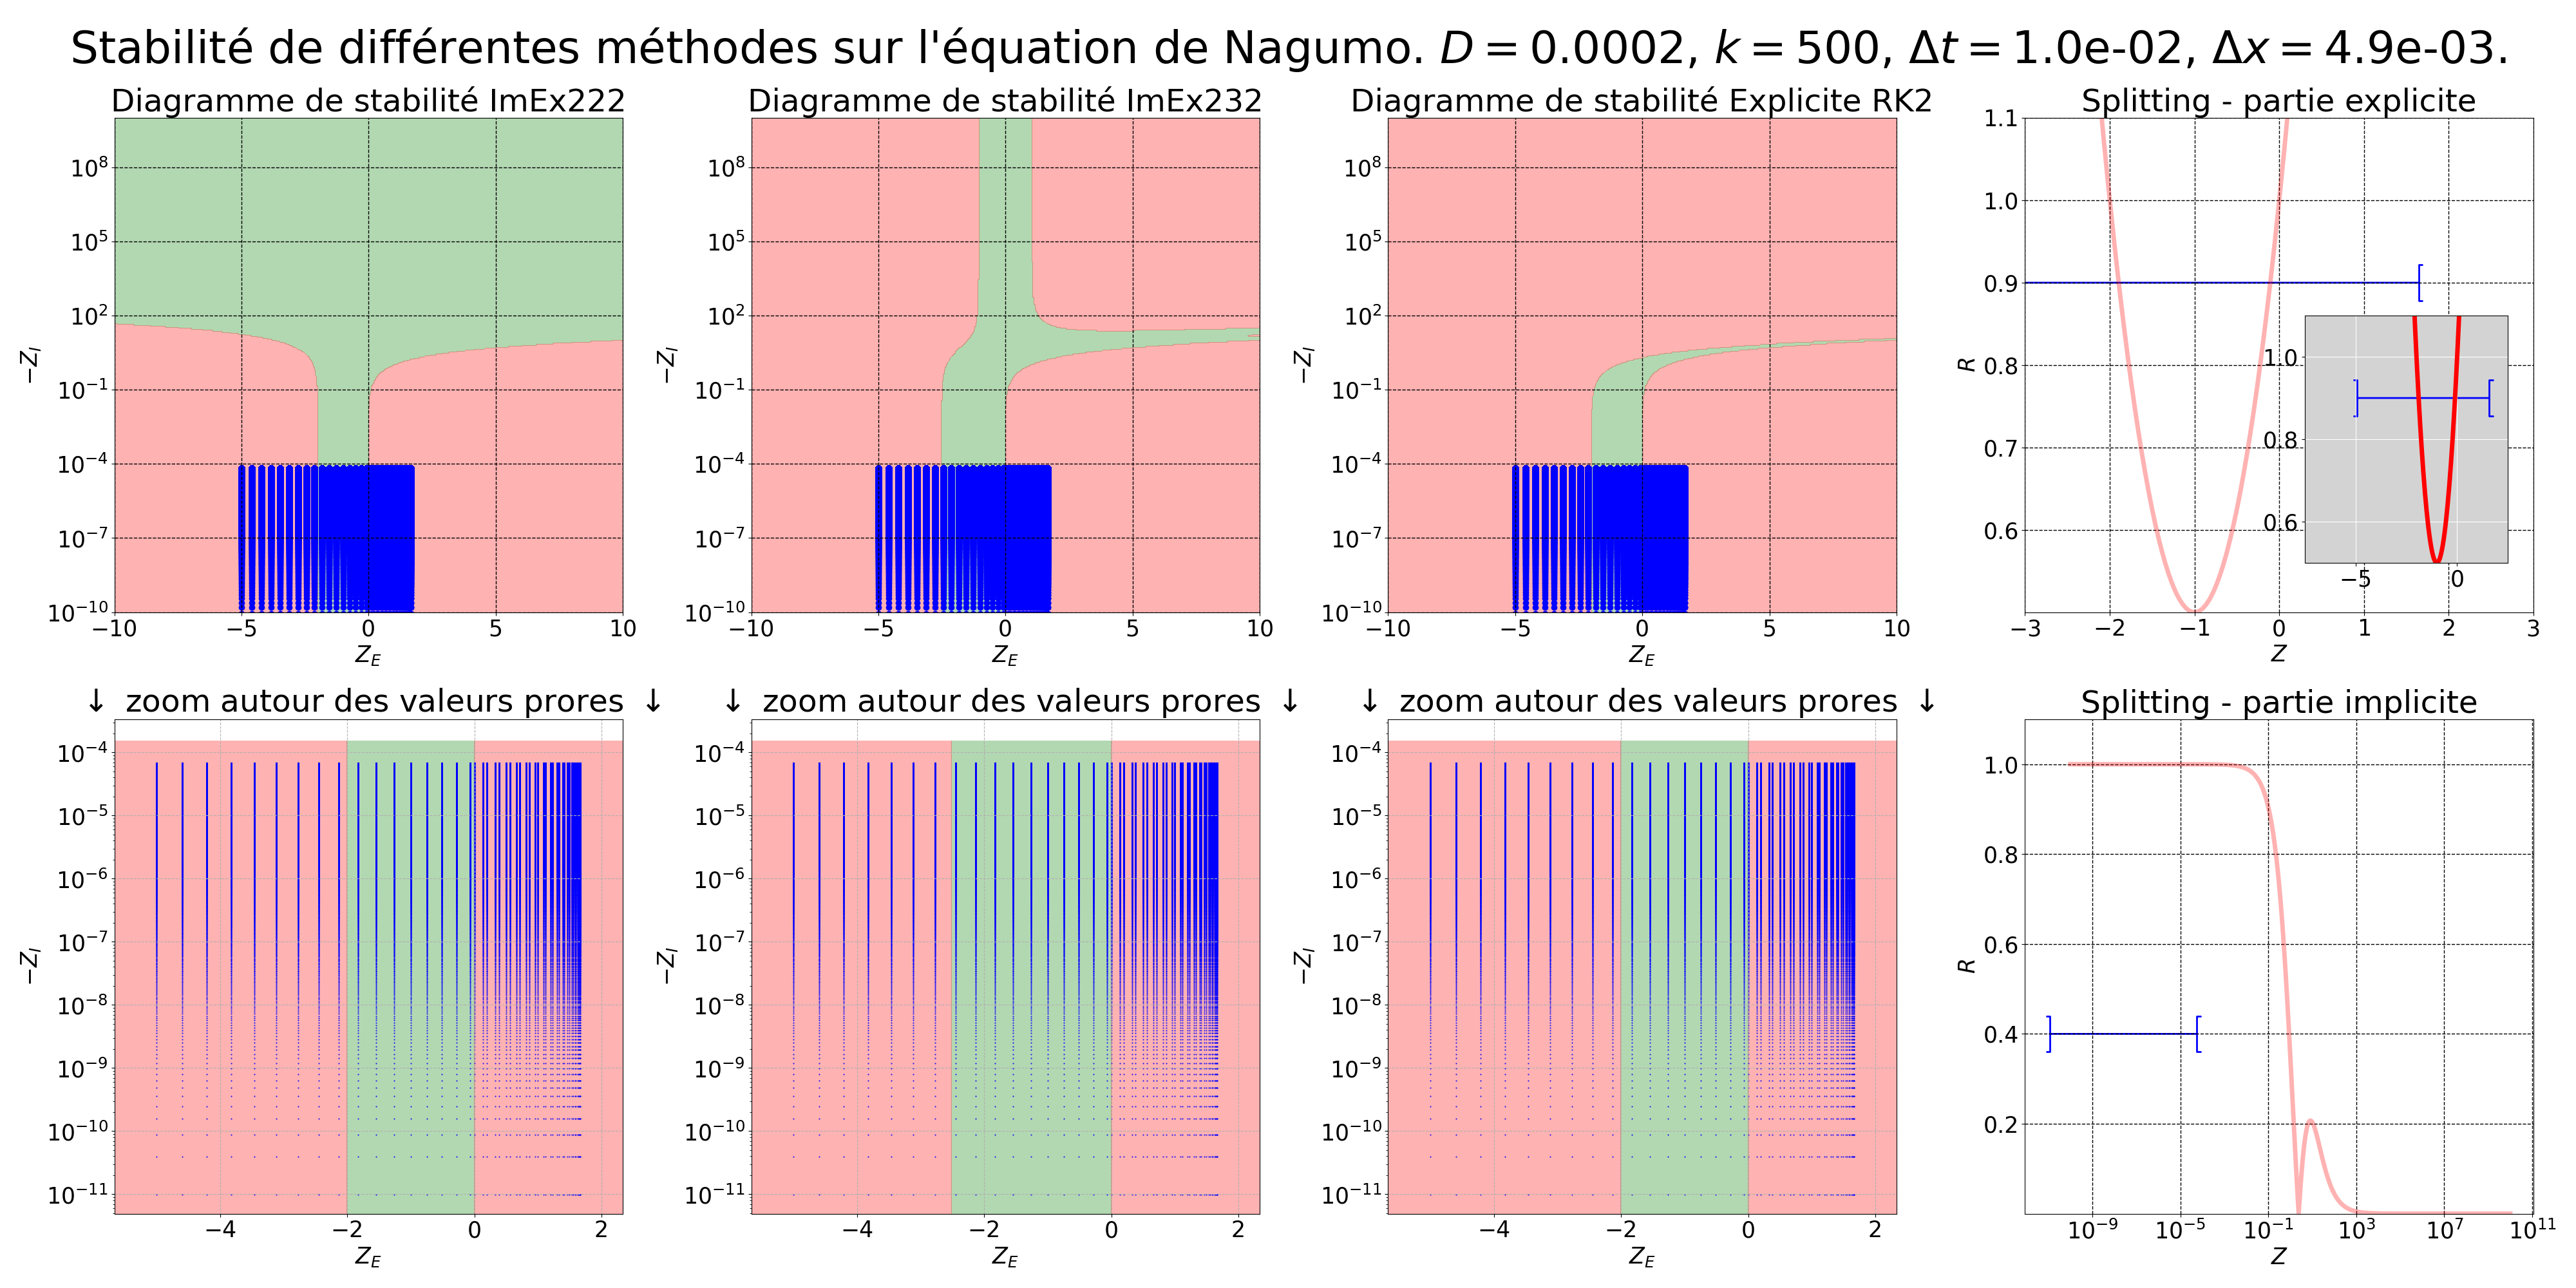
\includegraphics[width = \textwidth]{medias/2_/1_/STABILITE_D0.0002_k500_dt1.0e-02_dx4.9e-03.png}
\end{frame}
    \begin{frame}{Analyse de stabilité}{Annexe}
    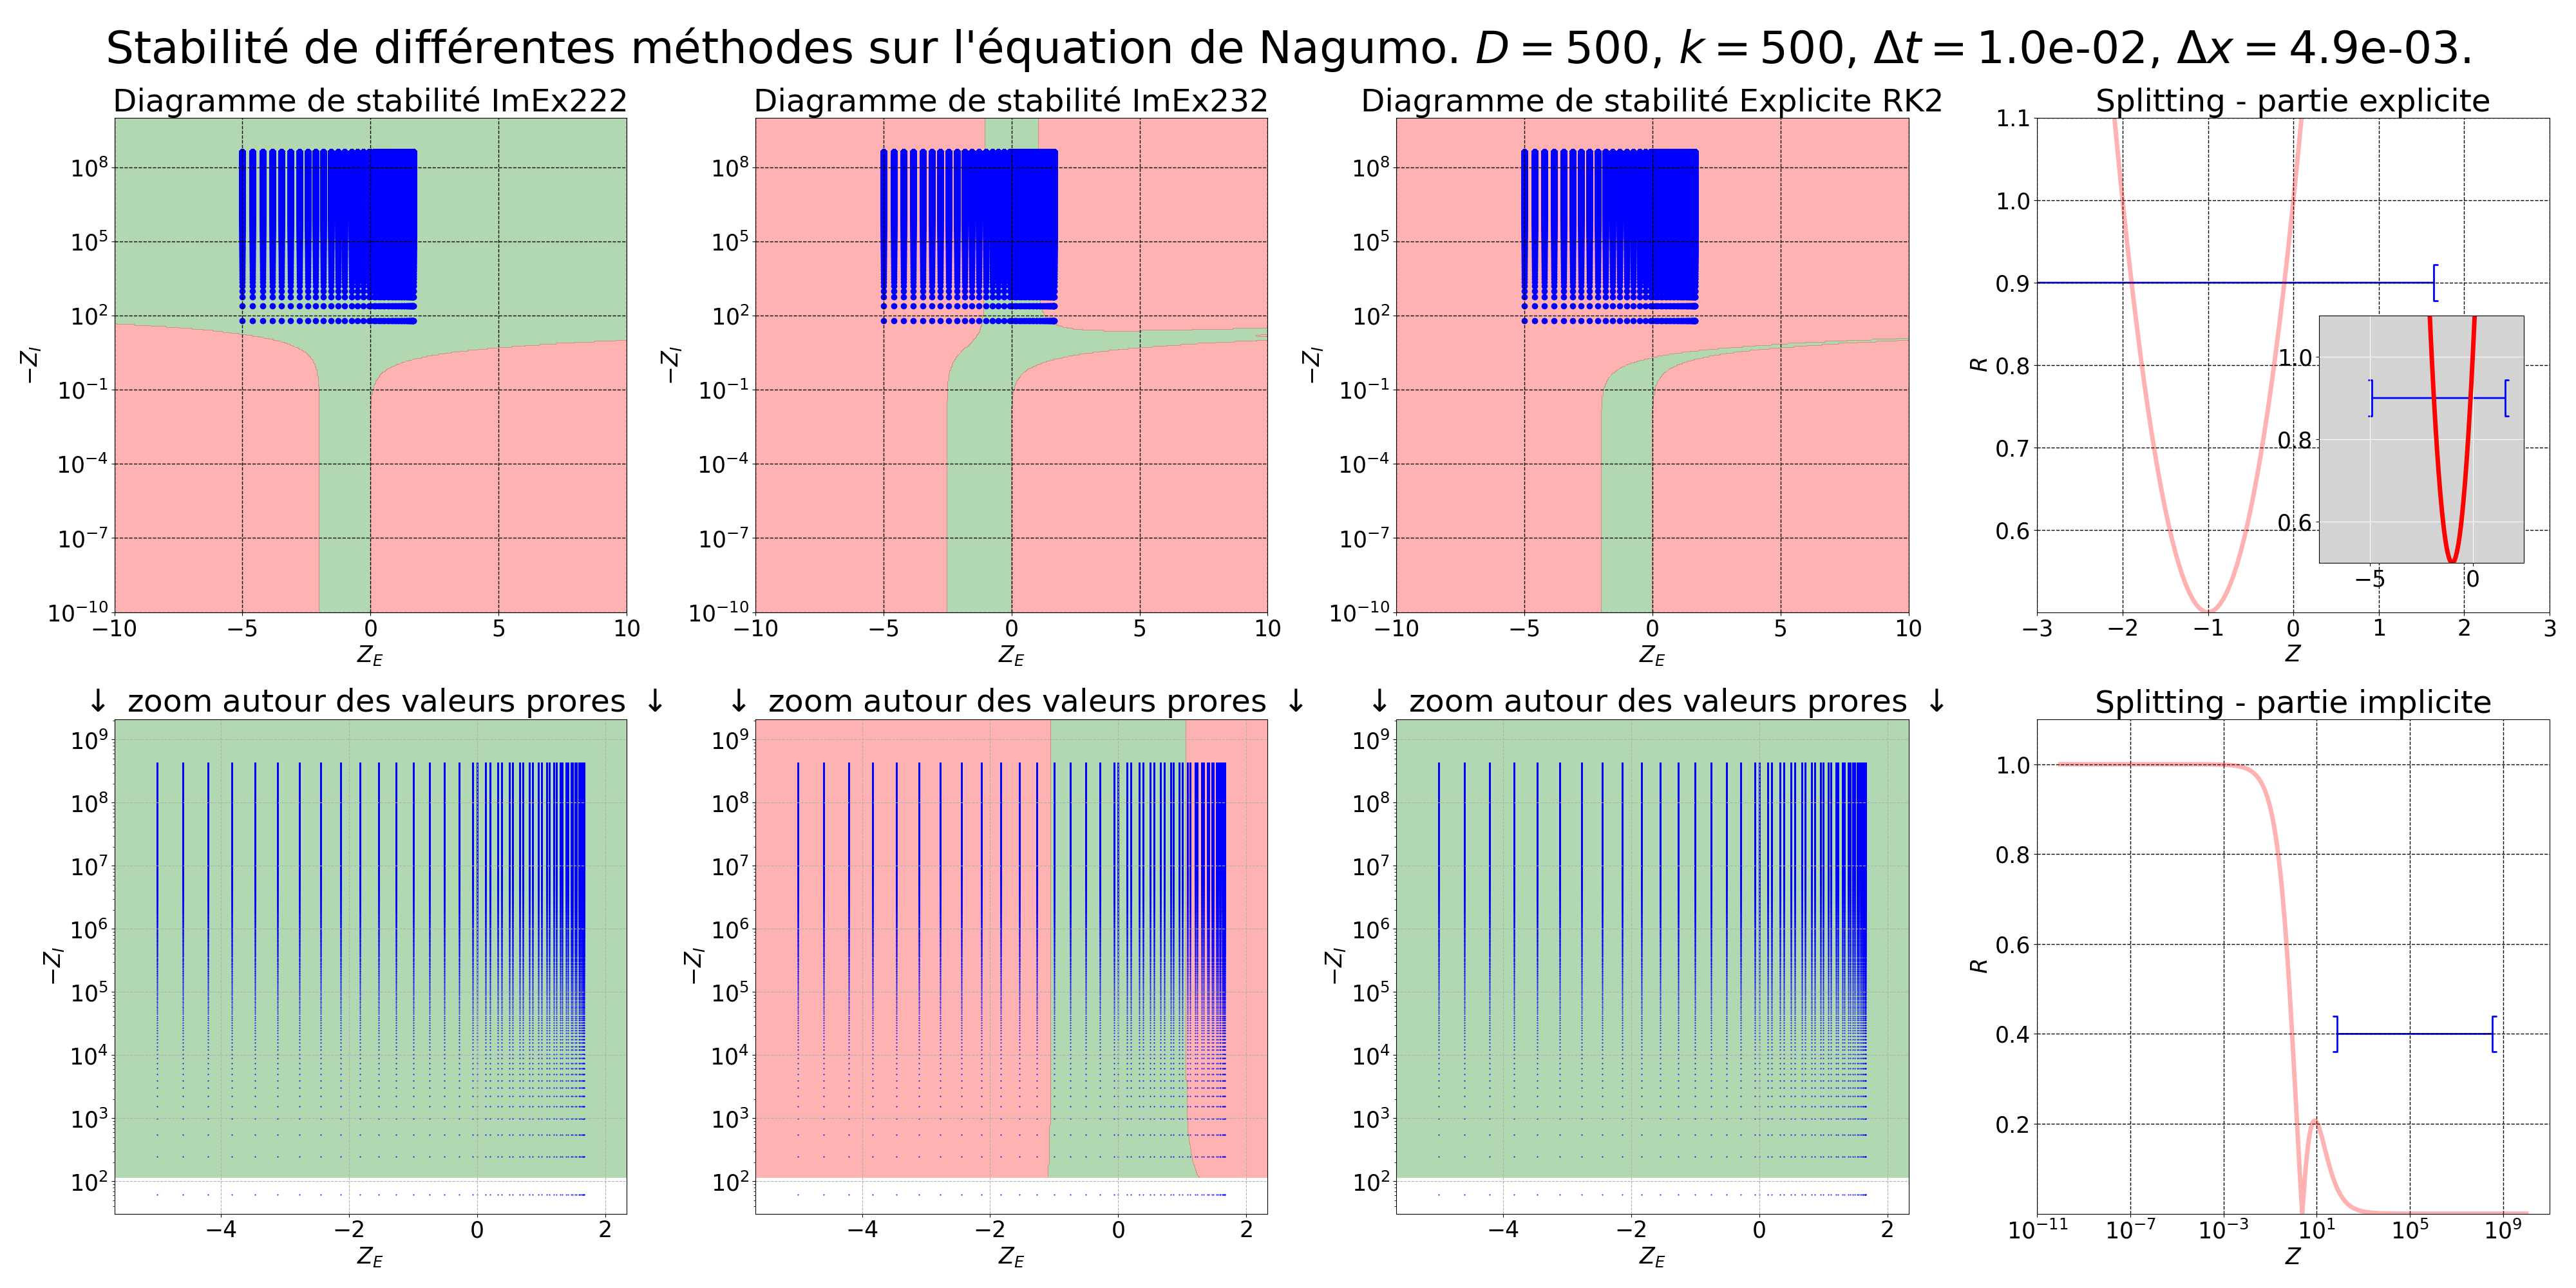
\includegraphics[width = \textwidth]{medias/2_/1_/STABILITE_D500_k500_dt1.0e-02_dx4.9e-03.png}
\end{frame}
  \begin{frame}{Contribution 1 | Comparaison ImEx - Splitting}{Convergence ($\emptyset$ MRA)}
    \begin{textblock*}{40pt}(0.7\paperwidth,0.2\paperheight)
        
\includegraphics[scale=.03]{medias/2_/1_/light_logo.png}
    \end{textblock*}

    \noindent\color{Primary}\rule{\linewidth}{0.6pt}\color{black}\\
    \textbf{Contexte:\\}
    \begin{itemize}
        \item $k=10$, $D=0.1$,
        \item $\Delta x = 2.4 \, 10^{-3}$,
        \item conditions de Neumann au bord (quasi infini).
    \end{itemize}
    \noindent\color{Primary}\rule{\linewidth}{0.6pt}\color{black}\\
    \centering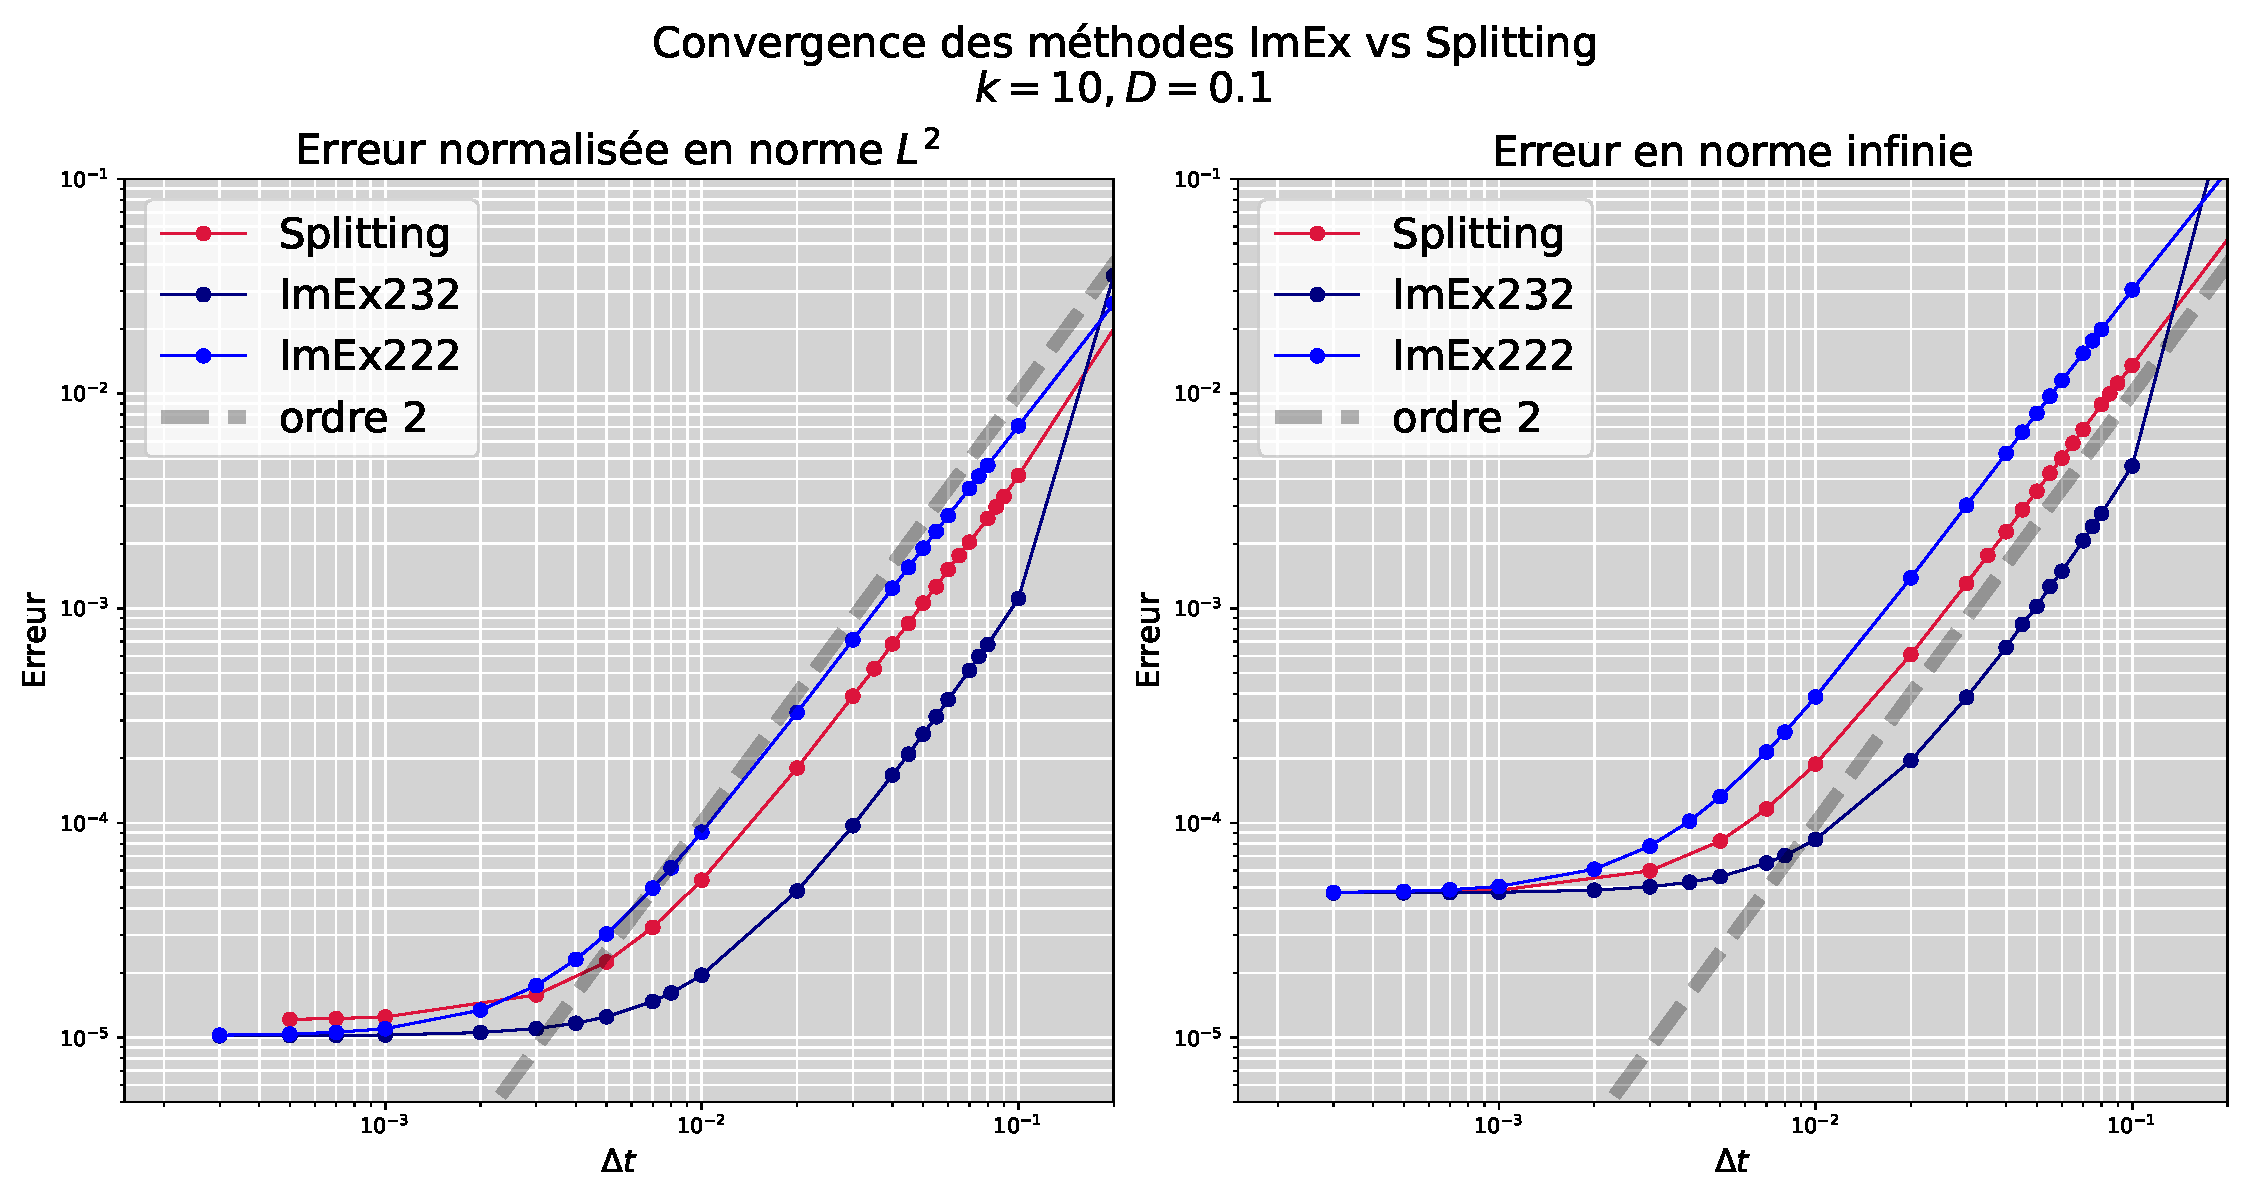
\includegraphics[width =.65 \textwidth]{ medias/2_/1_/ImEx_vs_splitting_k10_D0.1.pdf}
\end{frame}

  \begin{frame}{Contribution 1 | Comparaison ImEx - Splitting}{Convergence (avec MRA)}
    \begin{textblock*}{40pt}(0.7\paperwidth,0.2\paperheight)
        
\includegraphics[scale=.03]{medias/2_/1_/light_logo.png}
    \end{textblock*}
    \noindent\color{Primary}\rule{\linewidth}{0.6pt}\color{black}\\
    \textbf{Contexte:\\}
    \begin{itemize}
        \item $k=10$, $D=0.1$,
        \item Solution représentée du 12 $(\Delta x = 9\, 10^{-3})$ à 6,
        \item conditions de Neumann au bord (quasi infini).
    \end{itemize}   
    \noindent\color{Primary}\rule{\linewidth}{0.6pt}\color{black}\\

    \centering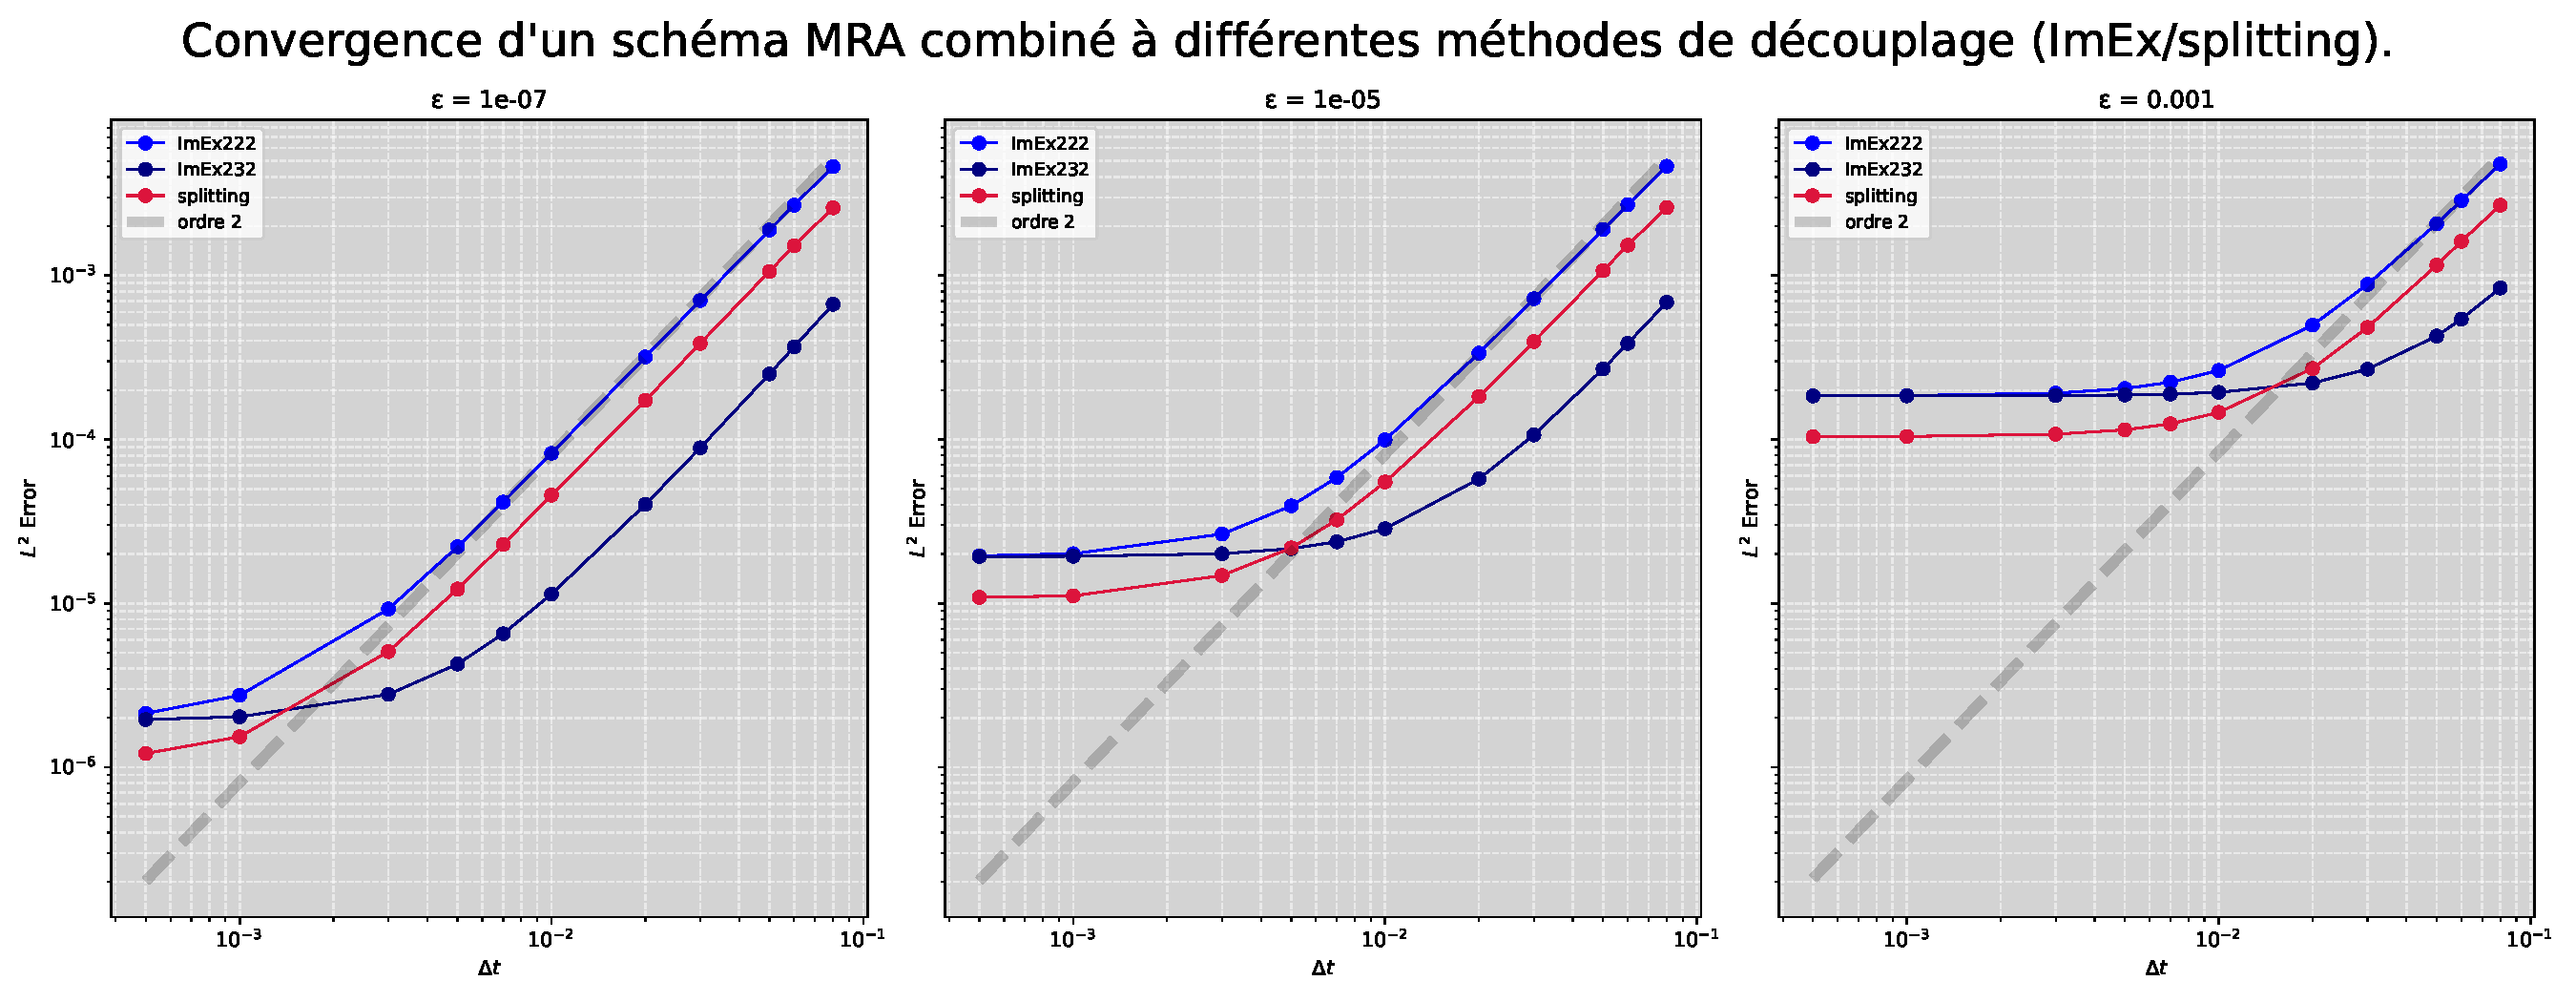
\includegraphics[width = .8\textwidth]{ medias/2_/1_/couplage_MRA_temps_k10_D01.pdf }
\end{frame}
  \input{slides/2_contributions/1_contrib/6_Conclusion}
\section{$2^{\text{ème}}$ contribution}
  Ce préambule mathématique présente divers concepts innervant dans les travaux du stage (chapitre \ref{par:contrib}). Le lecteur habitué peut ignorer ce chapitre et 
le consulter ponctuellement au besoin. Les sujets suivants y sont introduits:
\begin{enumerate}
    \item
    \item
    \item
    \item
    \item
\end{enumerate}
  \begin{frame}{Les deux approches de MRA}{Contribution 2 | Équations Modifiées, diffusion et MRA}
    
    \centering
    \begin{tikzpicture}[scale = 0.7]
    \foreach \i in {0,...,15}{
        \draw[fill=green!10] ({\i},3) rectangle ({((\i+1))},2);
    }
    \foreach \i in {1,...,15}{
        \draw[cyan, thick, ->,visible on=<2->](\i,2.7) -- (\i + 0.4,2.2);
        \draw[cyan, thick, ->,visible on=<2->](\i,2.7) --  (\i - 0.4 ,2.2);
    }

    \foreach \i in {0,...,1}{
        \draw[fill=green!10,visible on=<3->] ({8*\i},0) rectangle ({8*(\i+1)},1);}
    \foreach \i in {0,...,3}{
        \draw[fill=black!10,visible on=<3->] ({4*\i},-1) rectangle ({4*(\i+1)},0);}

    \foreach \i in {0,...,7}{
        \draw[fill=black!10,visible on=<3->] ({2*\i},-2) rectangle ({2*(\i+1)},-1);}

    \foreach \i in {0,...,15}{
        \draw[fill=black!10,visible on=<3->] ({\i},-3) rectangle ({((\i+1))},-2);}
    \draw[black, very thick, <->, visible on=<3->]
    (-.5,-3) -- (-.5,1)
    node[midway, left] {$\Delta l$};

    \draw[Primary, very thick, ->,visible on=<4->] (7.9,.9) -- (4,.5);
    \draw[Primary, very thick, ->,visible on=<4->] (8.1,.9) -- (12,.5);
    \node[right,visible on=<4->] at (0,4) {\textbf{Prédicteur polynomial à trois points.}};
    
    \draw[fill=red!10,visible on=<5->] (7,-3) rectangle (8,-2);
    \draw[fill=red!10,visible on=<5->] (8,-3) rectangle (9,-2);
    \draw[red, very thick, ->,visible on=<5->] (7.9,.2) -- (7.75,-2.5);
    \draw[red, very thick, ->,visible on=<5->] (8.1,.2) -- (8.25,-2.5);
    

    \draw[fill=orange!10,visible on=<6->] (8,-1) rectangle (4,0);
    \draw[fill=orange!10,visible on=<6->] (8,-1) rectangle (12,0);
    \draw[orange, very thick, ->,visible on=<6->] (7.9,.5) -- (6,-.5);
    \draw[orange, very thick, ->,visible on=<6->] (8.1,.5) -- (10,-.5);
    \draw[red, very thick, ->,visible on=<6->] (7.9,.2) -- (7.75,-2.5);
    \draw[red, very thick, ->,visible on=<6->] (8.1,.2) -- (8.25,-2.5);
    \node[right] at (-5,3) {\textbf{Flux numériques :}};
    \node[right] at (-5,2) {$\Phi_k^+ = \frac{u_{k+1} - u_k}{\Delta x}$};
    \node[right] at (-5,1) {$\Phi_k^- = \frac{u_{k} - u_{k-1}}{\Delta x}$};
    % \draw[black, very thick] (4,0) -- (4,1) node[pos=1, above] {interface d'intérêt};
        % \node[left] at (-.2,.5) {niveau $l$ (niveau courant)};
        % \node[left] at (-.2,-.5) {niveau $l+1$ };
        % \node[left] at (-.2,-1.5) {niveau $l+2$};
        % \node[left] at (-.2,-2.5) {niveau $l+3$ (ici, le niveau le plus fin)};

    \draw[cyan, very thick,->,visible on=<2->] (8.5,-3.3) -- (10,-3.3) node[pos=0,  left] {Pas d'adaptation};
    \draw[Primary, very thick,->,visible on=<4->] (8.5,-3.8) -- (10,-3.8) node[pos=0,  left] {MRA sans reconstruction des flux.};
    \draw[red, very thick,->,visible on=<5->] (8.5,-4.3) -- (10,-4.3) node[pos=0,  left] {MRA avec reconstruction des flux au niveau le plus fin.};
    \draw[orange, very thick,->,visible on=<6->] (8.5,-4.8) -- (10,-4.8) node[pos=0,  left] {MRA avec reconstruction des flux au niveau le plus proche.};
\end{tikzpicture}
\end{frame}
  \begin{frame}{Méthode d'obtention des équations modifiées}{Contribution 2 | Équations Modifiées, diffusion et MRA}
    \noindent\color{Primary}\rule{\linewidth}{0.6pt}\color{black}\\
    \textbf{Méthode d'obtention des équations modifiées :} Automatisation via \raisebox{-.5\height}{
\includegraphics[scale=0.05]{medias/2_/2_/sympy.png}}\\
% Préambule :
% \usepackage{tikz}
% \usetikzlibrary{arrows.meta,positioning}

\begin{tikzpicture}[
  >=Latex,
  node distance=1cm,
  every node/.style={font=\scriptsize},
  mystep/.style={
    rounded corners,
    draw=black,
    thick,
    align=center,
    inner sep=6pt,
    text width=3.7cm
  }
]

% Étape 1
\node[mystep, fill=Primary!20] (s1) {
  \textbf{Étape 1\\Développement de Taylor}\\
  $u_{k+\delta_x}^{\,n+\delta_t}
  \leftrightarrow
  u(x+\delta_x\,\Delta x,\;t+\delta_t\,\Delta t)$\\
  Développer en série de Taylor autour de $(x,t)$.
};

% Étape 2
\node[mystep, fill=Primary!40, right=of s1] (s2) {
  \textbf{Étape 2\\Cauchy-Kovalevskaya}\\
  Remplacer $\partial_t^k$ par $\partial_{xx}^p$ via l'EDP :\\
  $\partial_t u = D\,\partial_{xx}u$\\
  $\Rightarrow \partial_t^{\,k}u = D^{k}\,\partial_{xx}^{\,2k}u.$
};

% Étape 3
\node[mystep, fill=Primary!60, right=of s2] (s3) {
  \textbf{Étape 3\\Relation $\Delta t  \leftrightarrow \Delta x$}\\
  Introduire $\displaystyle \lambda = \frac{D\,\Delta t}{\Delta x^{2}}$ (Von Neumann).
};

% Flèches
\draw[->, thick] (s1) -- (s2);
\draw[->, thick] (s2) -- (s3);
\end{tikzpicture}\\ \pause
    \noindent\color{Primary}\rule{\linewidth}{0.6pt}\color{black}\\
    \textbf{Multirésolution adaptative sans reconstruction des flux :}\\
    Remplacer $\Delta x$ par $2^{\Delta l} \Delta x$.\\ \pause
    \noindent\color{Primary}\rule{\linewidth}{0.6pt}\color{black}\\
    \textbf{Prise en compte de la reconstruction des flux :}\\
    \begin{itemize}
        \item Reconstruction : \small$\left[ u^{\overline l}_{2^{\Delta l}k-1} ,  u^{\overline l}_{2^{\Delta l}k}  ,  u^{\overline l}_{2^{\Delta l}k+1} ,  u^{\overline l}_{2^{\Delta l}k+2} \right]^T= P^{\Delta l} \left[ u^{\overline l- \Delta l}_{k-1} ,  u^{\overline l - \Delta l}_{k}  ,  u^{\overline l}_{k+1} ,  u^{\overline l - \Delta l}_{k+2} \right]^T$\normalsize
        \item Taille cellule : $2^{\Delta l} \Delta x$, Pas approximation gradient $\Delta x$ .
    \end{itemize}
\end{frame}
  
\begin{frame}{Contribution 2 | Équations Équivalentes, diffusion et MRA}{Résultats}
    \centering\scriptsize$\Delta l$ écart de niveau - $D>0$ coefficient de diffusion - $\Delta x$ pas spatial de la grille fine - $\Delta t$ pas temporel\\\normalsize
    \noindent\color{Primary}\rule{\linewidth}{0.6pt}\color{black}\\
    \textbf{Sans multirésolution adaptative: }\\
    \begin{center}\footnotesize
    \begin{align}
            \frac{\partial u}{\partial t}  =&D \frac{\partial^{2}u}{\partial x^{2}}
            + \Delta x^{2} \frac{D}{12}             \frac{\partial^{4}u}{\partial x^{4}} 
            -  \Delta t^{2} \frac{D^{3}}{6}          \frac{\partial^{6}u}{\partial x^{6}} 
            -  \Delta t^{3} \frac{D^{4}}{24}        \frac{\partial^{8}u}{\partial x^{8}}  + \mathcal{O}(\Delta x^4 , \Delta t^4).
    \end{align}
    \end{center}\pause
    \noindent\color{Primary}\rule{\linewidth}{0.6pt}\color{black}\\
    \textbf{Avec multirésolution adaptative - sans reconstruction des flux: }\\
        \begin{center}\footnotesize
        \begin{align}\label{eq:sansRecons:brute}
            \frac{\partial}{\partial t} u=
                D \frac{\partial^{2}u}{\partial x^{2}}
                + (2^{\Delta l} \Delta x)^{2}  \frac{D}{12} \frac{\partial^{4}u}{\partial x^{4}}
                -\Delta t^{2} \frac{D^{3}}{6}   \frac{\partial^{6}u}{\partial x^{6}}
                -\Delta t^{3} \frac{D^{4} }{24} \frac{\partial^{8}u}{\partial x^{8}}
                + \mathcal{O}(\Delta x^4 , \Delta t^4).
        \end{align}
        \end{center}\pause
    \noindent\color{Primary}\rule{\linewidth}{0.6pt}\color{black}\\
    \textbf{Avec multirésolution adaptative - avec reconstruction des flux: }\\
        \begin{center}\scriptsize
        \begin{align}\label{eq:equiv_brute_recons}
            \frac{\partial u}{\partial t} =&\; D \frac{\partial^2 u}{\partial x^2} 
            - \Delta t \frac{D^2}{2} \, \bigl( 2^{2\Delta l}- 1 \bigr)          \frac{\partial^4 u}{\partial x^4}
            - \Delta t^2\, \frac{D^3}{6}          \frac{\partial^6 u}{\partial x^6}
            - \Delta t^3\, \frac{D^4}{24}         \frac{\partial^8 u}{\partial x^8} 
            + \Delta x^2\, \frac{2^{2\Delta l}D}{12}  (1 - 3 \Delta l)  \frac{\partial^4 u}{\partial x^4}
            + \mathcal{O}(\Delta x^4 , \Delta t^4).
        \end{align}
    \end{center}

\end{frame}
  
\begin{frame}{Résultats}{Contribution 2 | Équations Modifiées, diffusion et MRA}
    \centering\scriptsize$\Delta l$ écart de niveau - $D>0$ coefficient de diffusion - $\Delta x$ pas spatial de la grille fine - $\lambda = D \frac{\Delta t}{\Delta x^2}$ $\mathrm{c}^\mathrm{ste}$ Von Neumann\\\normalsize
    \noindent\color{Primary}\rule{\linewidth}{0.6pt}\color{black}\\
    \textbf{Sans multirésolution adaptative: }\\
    \begin{center}\footnotesize
        \begin{align}\label{eq:ref:cfl}
            \frac{\partial u}{\partial t}  =&D \frac{\partial^{2}u}{\partial x^{2}}
            + \Delta x^{2} \frac{D}{12}             \frac{\partial^{4}u}{\partial x^{4}} 
            - \lambda^2 \Delta  x^{4} \frac{D}{6}          \frac{\partial^{6}u}{\partial x^{6}} 
            - \lambda^3 \Delta x^{6} \frac{D}{24}        \frac{\partial^{8}u}{\partial x^{8}}  + \mathcal{O}(\Delta x^7).
        \end{align}
    \end{center}\pause
    \noindent\color{Primary}\rule{\linewidth}{0.6pt}\color{black}\\
    \textbf{Avec multirésolution adaptative - sans reconstruction des flux: }\\
        \begin{center}\footnotesize
            \begin{align}\label{eq:sansRecons:cfl}
            \frac{\partial}{\partial t} u&=
                D \frac{\partial^{2}u}{\partial x^{2}}
                + (2^{\Delta l} \Delta x)^{2}  \frac{D}{12} \frac{\partial^{4}u}{\partial x^{4}}
                -\lambda^2 \Delta x^{4} \frac{D}{6}   \frac{\partial^{6}u}{\partial x^{6}}
                -\lambda^3 \Delta x^{6} \frac{D}{24} \frac{\partial^{8}u}{\partial x^{8}} + \mathcal{O}(\Delta x^7)
    \end{align}
        \end{center}\pause
    \noindent\color{Primary}\rule{\linewidth}{0.6pt}\color{black}\\
    \textbf{Avec multirésolution adaptative - avec reconstruction des flux: }\\
        \begin{center}\scriptsize
        \begin{align}\label{eq:equiv_cfl_recons}
            \frac{\partial u}{\partial t}
            =&+ D \frac{\partial^{2}u}{\partial x^{2}}
            + \Delta x^{2}\, D \, \Bigl( 
            \frac{\lambda}{2} (2^{2 \Delta l} - 1) + \frac{2^{2 \Delta l} }{12} (1 - 3 \Delta l)
            \Bigr)\frac{\partial^{4}u}{\partial x^{4}}\
            - \Delta x^{4} \frac{D \lambda^{2} \frac{\partial^{6}u}{\partial x^{6}}}{6} - \Delta x^{6} \frac{D \lambda^{3} \frac{\partial^{8}u}{\partial x^{8}}}{24}
            + \mathcal{O}(\Delta x^7). 
        \end{align}

        \end{center}

\end{frame}
  \begin{frame}{Conclusion}{Contribution 2 | Équations Modifiées, diffusion et MRA}
    \textbf{Apprentissage personnel : }\\
    \begin{itemize}
        \item Calcul formel grâce à la libraire Sympy.
        \item Développement de la compréhension de l'algorithme d'adaptation.
        \item Usage des \emph{équations Modifiées} comme puissant outil d'analyse, dans la continuité de l'équipe hpc@maths \cite{Massot2025_meshAdaptation,belloti_et_al_2025}.
    \end{itemize}
    \noindent\color{Primary}\rule{\linewidth}{0.6pt}\color{black}\\
    \textbf{Résultats}\\
        \begin{itemize}
            \item \textbf{Développement d'équations équivalente} pour un schéma diffusif avec plusieurs types d'adaptation
            permettant une mise en lumière de l'erreur pour chaque contexte.\\
            \scriptsize{(sans MRA, MRA sans reconstruction des flux et MRA avec reconstruction des flux)}
            \item \textbf{La reconstruction semble ajouter plus de termes d'erreurs}\\\scriptsize{+ potentiellement perte d'ordre (à confirmer).}
        \end{itemize}
\end{frame}
\section{$3^{\text{ème}}$ contribution}
  Ce préambule mathématique présente divers concepts innervant dans les travaux du stage (chapitre \ref{par:contrib}). Le lecteur habitué peut ignorer ce chapitre et 
le consulter ponctuellement au besoin. Les sujets suivants y sont introduits:
\begin{enumerate}
    \item
    \item
    \item
    \item
    \item
\end{enumerate}
  \begin{frame}{Contribution 3 | Étude nnumérique, diffusion et MRA}{Intégration avec ERK2}
    \begin{center}
        \begin{tabular}
            {|c|c|c|}\hline Schéma $n^o$ & Niveau d'évaluation des flux & Erreur $L^2$ \\\hline\texttt{I} & $\emptyset$ MRA & $2 \times 10^{-5}$ \\\texttt{II} & Courant & $1 \times 10^{-4}$ \\\texttt{III} & Plus fin $l^{\max}$& $3 \times 10^{-4}$ \\\texttt{IV} & Inférieur direct ($l+1$) & $2 \times 10^{-4}$ \\\hline
        \end{tabular}
    \end{center}
\end{frame}
  \begin{frame}{Contribution 3 | Étude nnumérique, diffusion et MRA}{Analyse Stabilité ?}
    \centering \Large
    \href{https://github.com/Ocelot-Pale/etude_MR_RK2}{\color{Primary} \underline{Etude de stabilité}}\color{black}
\end{frame}
  \begin{frame}{Intégration avec ROCK2}{Contribution 3 | Étude numérique, diffusion et MRA}

    \begin{textblock*}{40pt}(0.1\paperwidth,0.87\paperheight)
        
\includegraphics[scale=.03]{medias/2_/1_/light_logo.png}
    \end{textblock*}
    \centering
    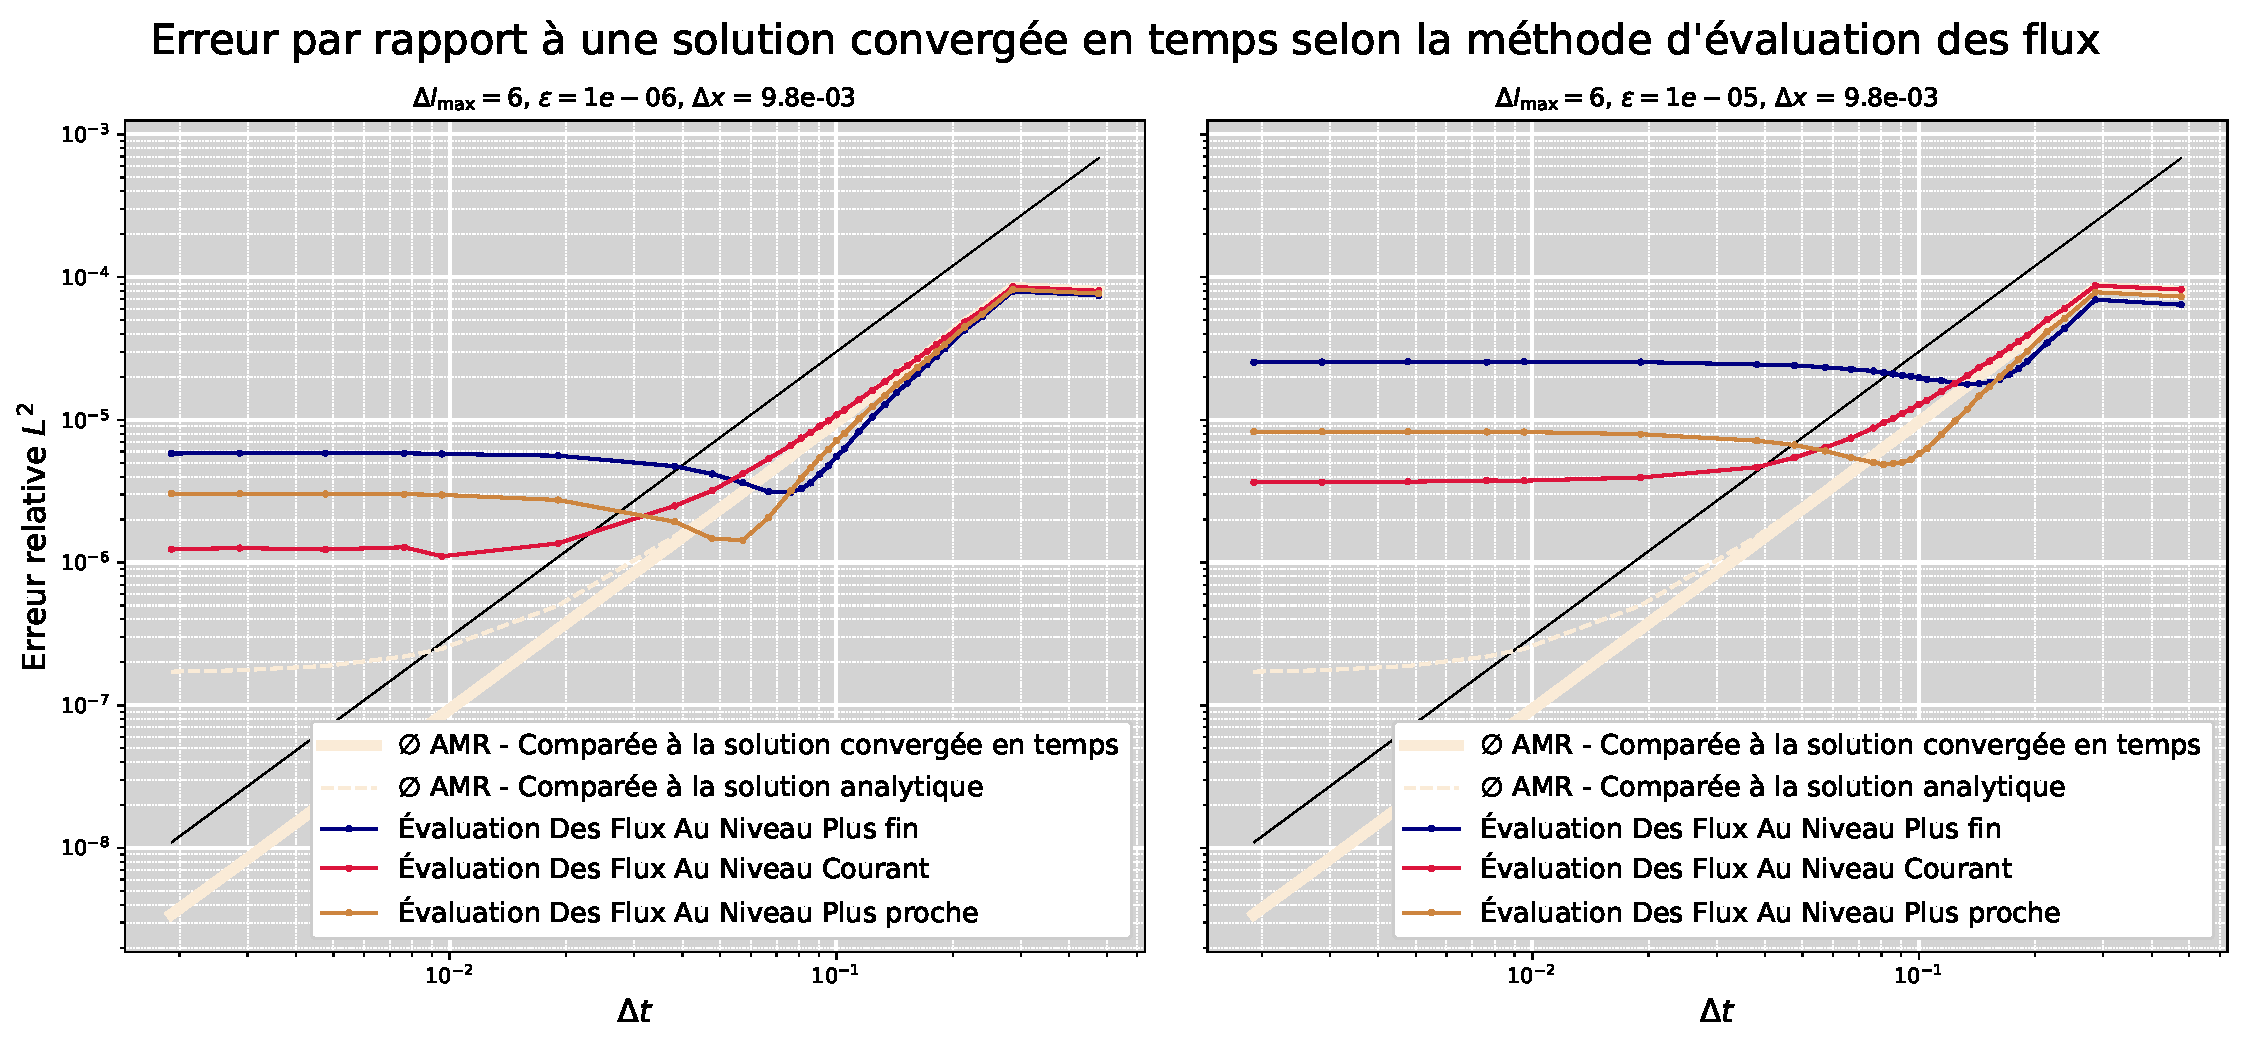
\includegraphics[width= .9\textwidth]{medias/2_/3_/flux_reconstruction_method_diffusion.pdf}
        \visible<2->{\scriptsize{\vspace{-1.75em}\begin{align}\label{eq:equiv_cfl_recons}
            \frac{\partial u}{\partial t}
            =&+ D \frac{\partial^{2}u}{\partial x^{2}}
            + \Delta x^{2}\, D \, \Bigl( 
            \frac{\lambda}{2} (2^{2 \Delta l} - 1) + \frac{2^{2 \Delta l} }{12} (1 - 3 \Delta l)
            \Bigr)\frac{\partial^{4}u}{\partial x^{4}}\
            - \Delta x^{4} \frac{D \lambda^{2} \frac{\partial^{6}u}{\partial x^{6}}}{6} - \Delta x^{6} \frac{D \lambda^{3} \frac{\partial^{8}u}{\partial x^{8}}}{24}
            + \mathcal{O}(\Delta x^7). 
        \end{align}}}
    \begin{textblock*}{40pt}(0.2\paperwidth,0.96\paperheight)
        {\color{black}{+ Ponio}}
    \end{textblock*}
    \href{https://github.com/Ocelot-Pale/etude_MR_RK2}{\color{Primary} \underline{Visualisation de la distribution des erreurs.}}\color{black}
\end{frame}

  \begin{frame}{Contribution 3 | Étude nnumérique, diffusion et MRA}{Profils d'erreur}
    \centering
    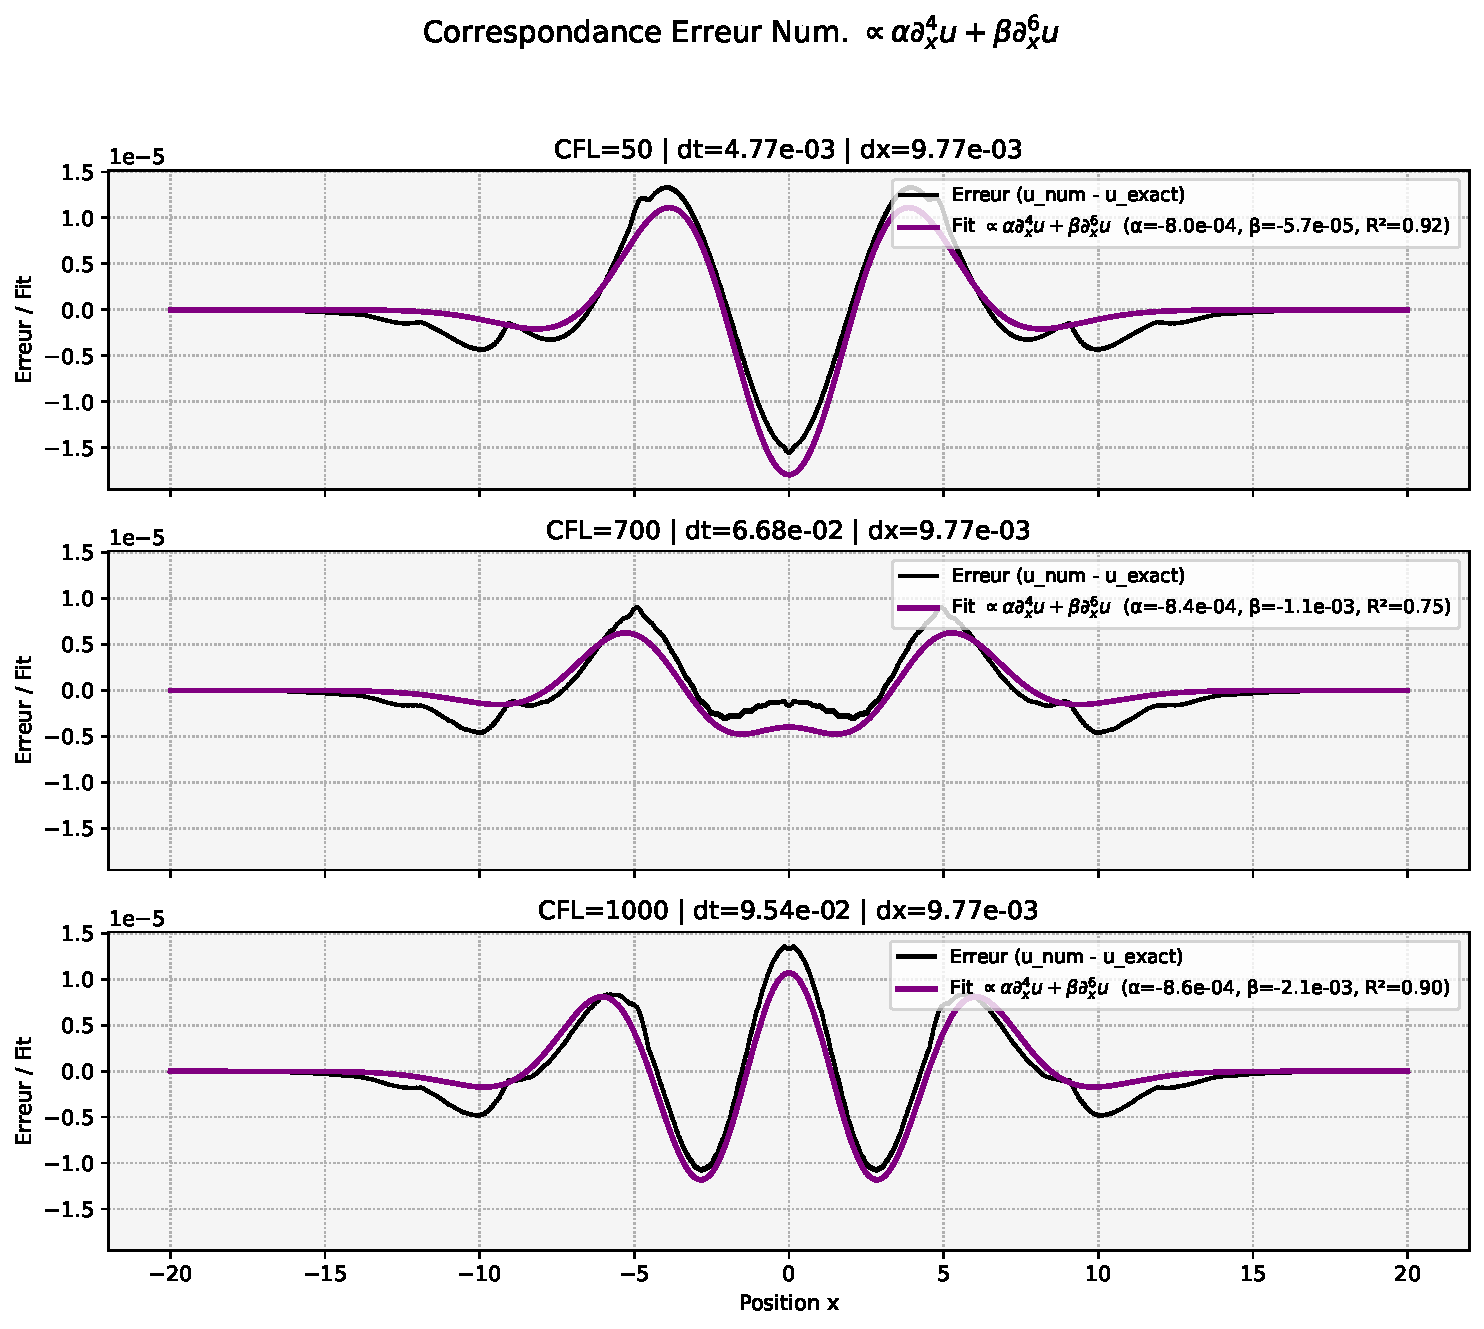
\includegraphics[height= .85\textheight]{medias/2_/3_/derivees_spatiales_VS_err_num.pdf}
    
\end{frame}
  \begin{frame}{Explications}{Contribution 3 | Étude numérique, diffusion et MRA}
    \noindent\color{Primary}\rule{\linewidth}{0.6pt}\color{black}\\
        \textbf{Chute prématurée de l'erreur: }\\
        Les dérivées $\partial_x^{4}$ et  $\partial_x^{6}$ ont des poids différents dans l’erreur selon la constante de Von Neumann $\lambda$.
        Leurs profils se "compensent" quand elles ont un poids comparable.
    \noindent\color{Primary}\rule{\linewidth}{0.6pt}\color{black}\\
        \textbf{Moins bonne performances quand l'erreur temporelle est faible}\\
            Plus de termes d'erreur dans la contribution dominante de l'erreur : 
            \begin{center}
                \renewcommand{\arraystretch}{1}
                \begin{tabular}{@{}clc@{}}
                    \toprule
                    \textbf{Schéma n\textsuperscript{o}} & \textbf{Évaluation des flux} &
                    \makecell[c]{\textbf{Constante pondérant l'erreur en $\Delta x^{2}\,\partial_{x}^{4}u$}\\
                                \textbf{(dominante quand $\lambda$ est petite)}} \\
                    \midrule
                    I   & $\varnothing$ AMR          & $\dfrac{D}{12}$ \\[1mm]
                    II  & Sans reconstruction         & $2^{\Delta l}\,\dfrac{D}{12}$ \\[1mm]
                    III & Avec reconstruction         &
                        $D\,\Bigl(\dfrac{\lambda}{2}\,(2^{2\Delta l}-1)
                        + \dfrac{2^{2\Delta l}}{12}\,(1-3\Delta l)\Bigr)$ \\[1mm]
                    \bottomrule
                \end{tabular}
            \end{center}
\end{frame}
  \begin{frame}{Contribution 3 | Étude nnumérique, diffusion et MRA}{Conclusion}
    \begin{itemize}
    \item La reconstruction semble ici problème car : prédicteur polynomial précis à l'ordre 3, permet une évaluation des 
        gradients à l'ordre 2. Or le schéma est d'ordre 2, donc erreur de prédiction du même ordre et s'accumule.
    \end{itemize}
\end{frame}
\section{Compléments}
% \begin{frame}{Essais numériques - prédicteur à 5 points}{Complément}
    \centering{
    \noindent\color{Primary}\rule{\linewidth}{0.6pt}\\
    \textbf{État initial\\}\color{black}\scriptsize
    \begin{itemize}
        \item Condition de Naumann,
        \item $\varepsilon = 5\,10^{-7}$,
        \item Niveaux 12 à 4, $\Delta x = 40/2^{12} \approx 9 \, 10^{-3}$,
        \item Comparaison à une solution convergée en temps $\Delta t = 10^{-7}$.
    \end{itemize}
    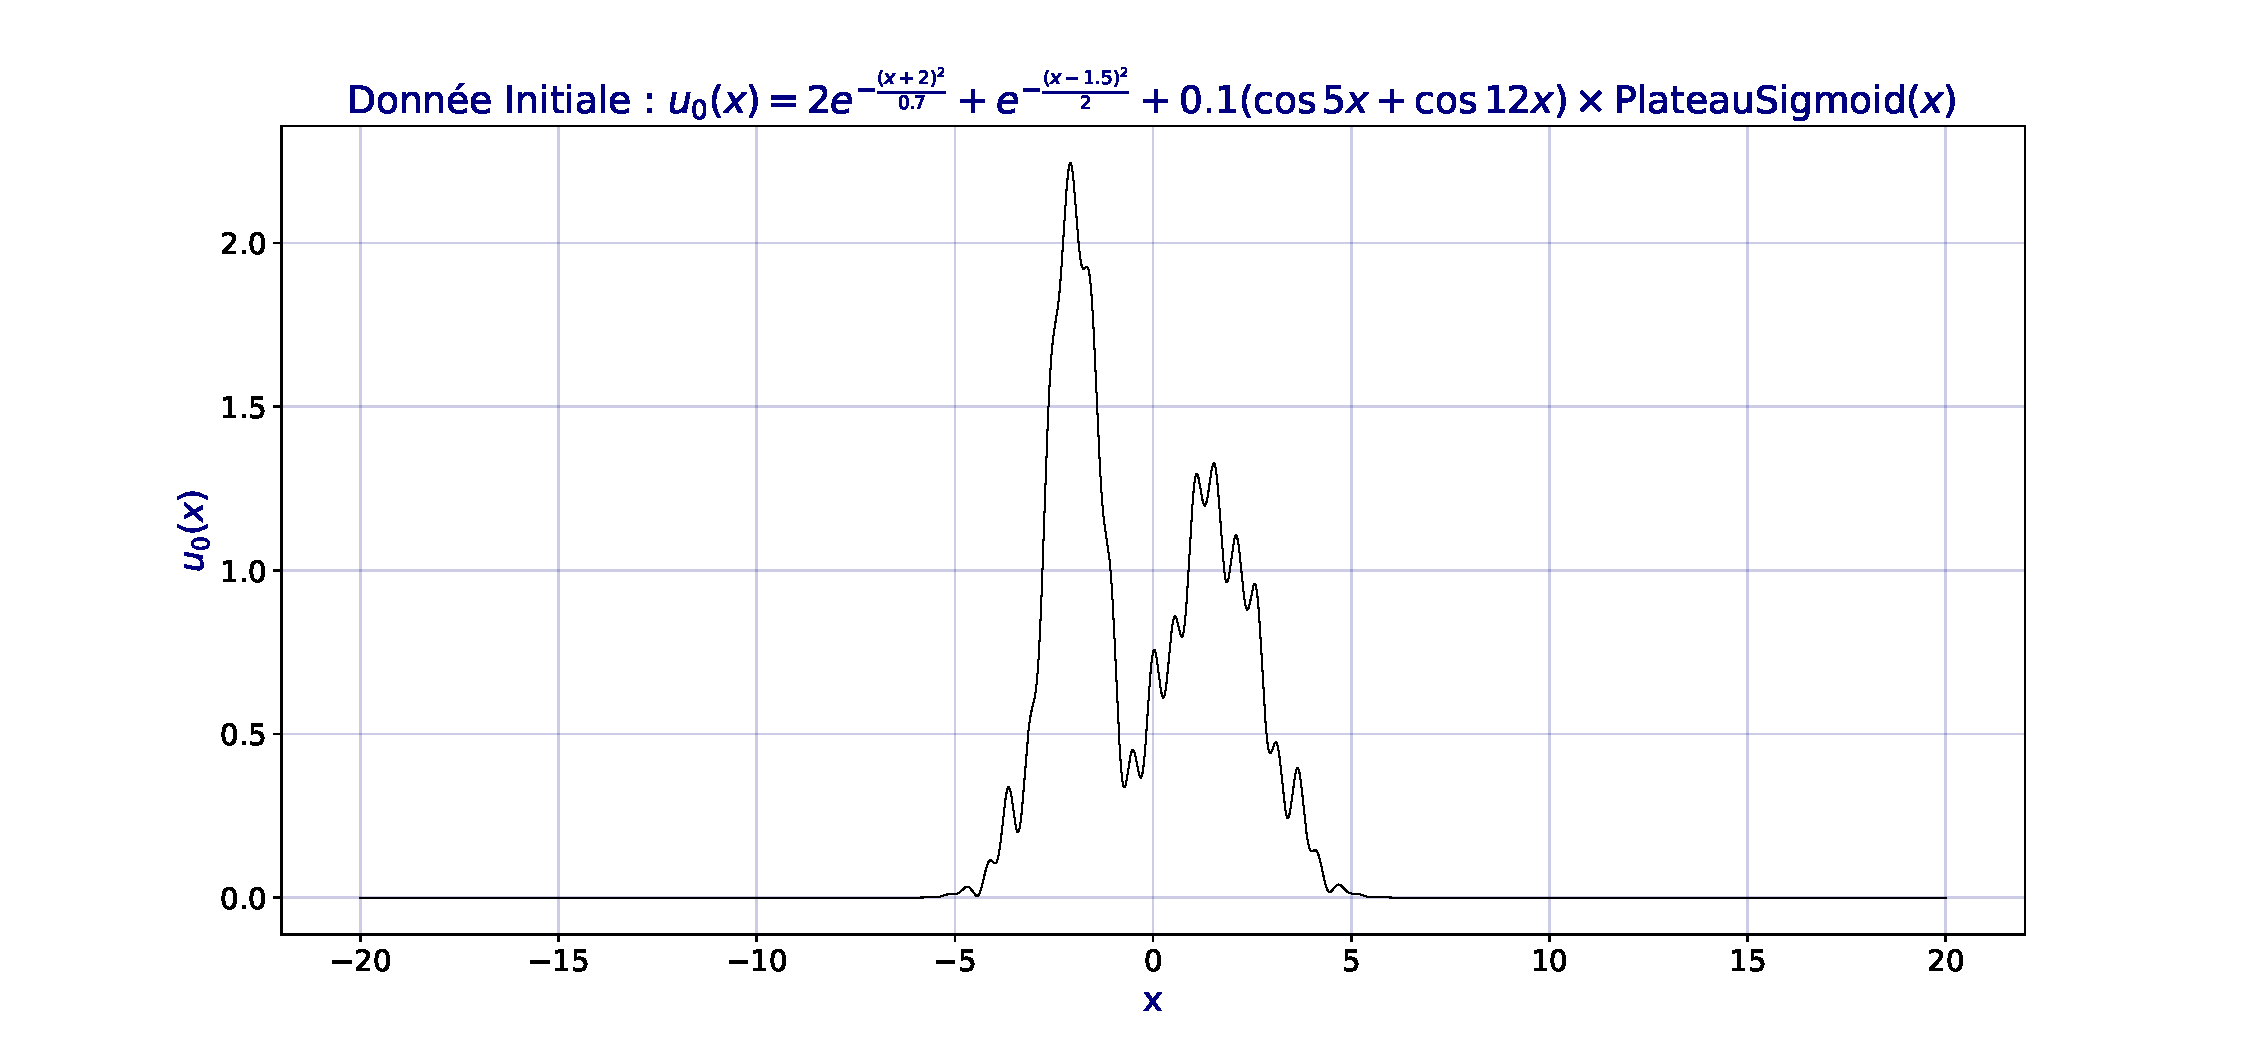
\includegraphics[width = .85\textwidth]{medias/3_/cas_test.pdf}}
\end{frame}
\begin{frame}{Complément}{Essais numériques - prédicteurs à 5 points}
    \begin{textblock*}{40pt}(0.05\paperwidth,0.88\paperheight)
\includegraphics[scale=.03]{medias/2_/1_/light_logo.png}\end{textblock*}
    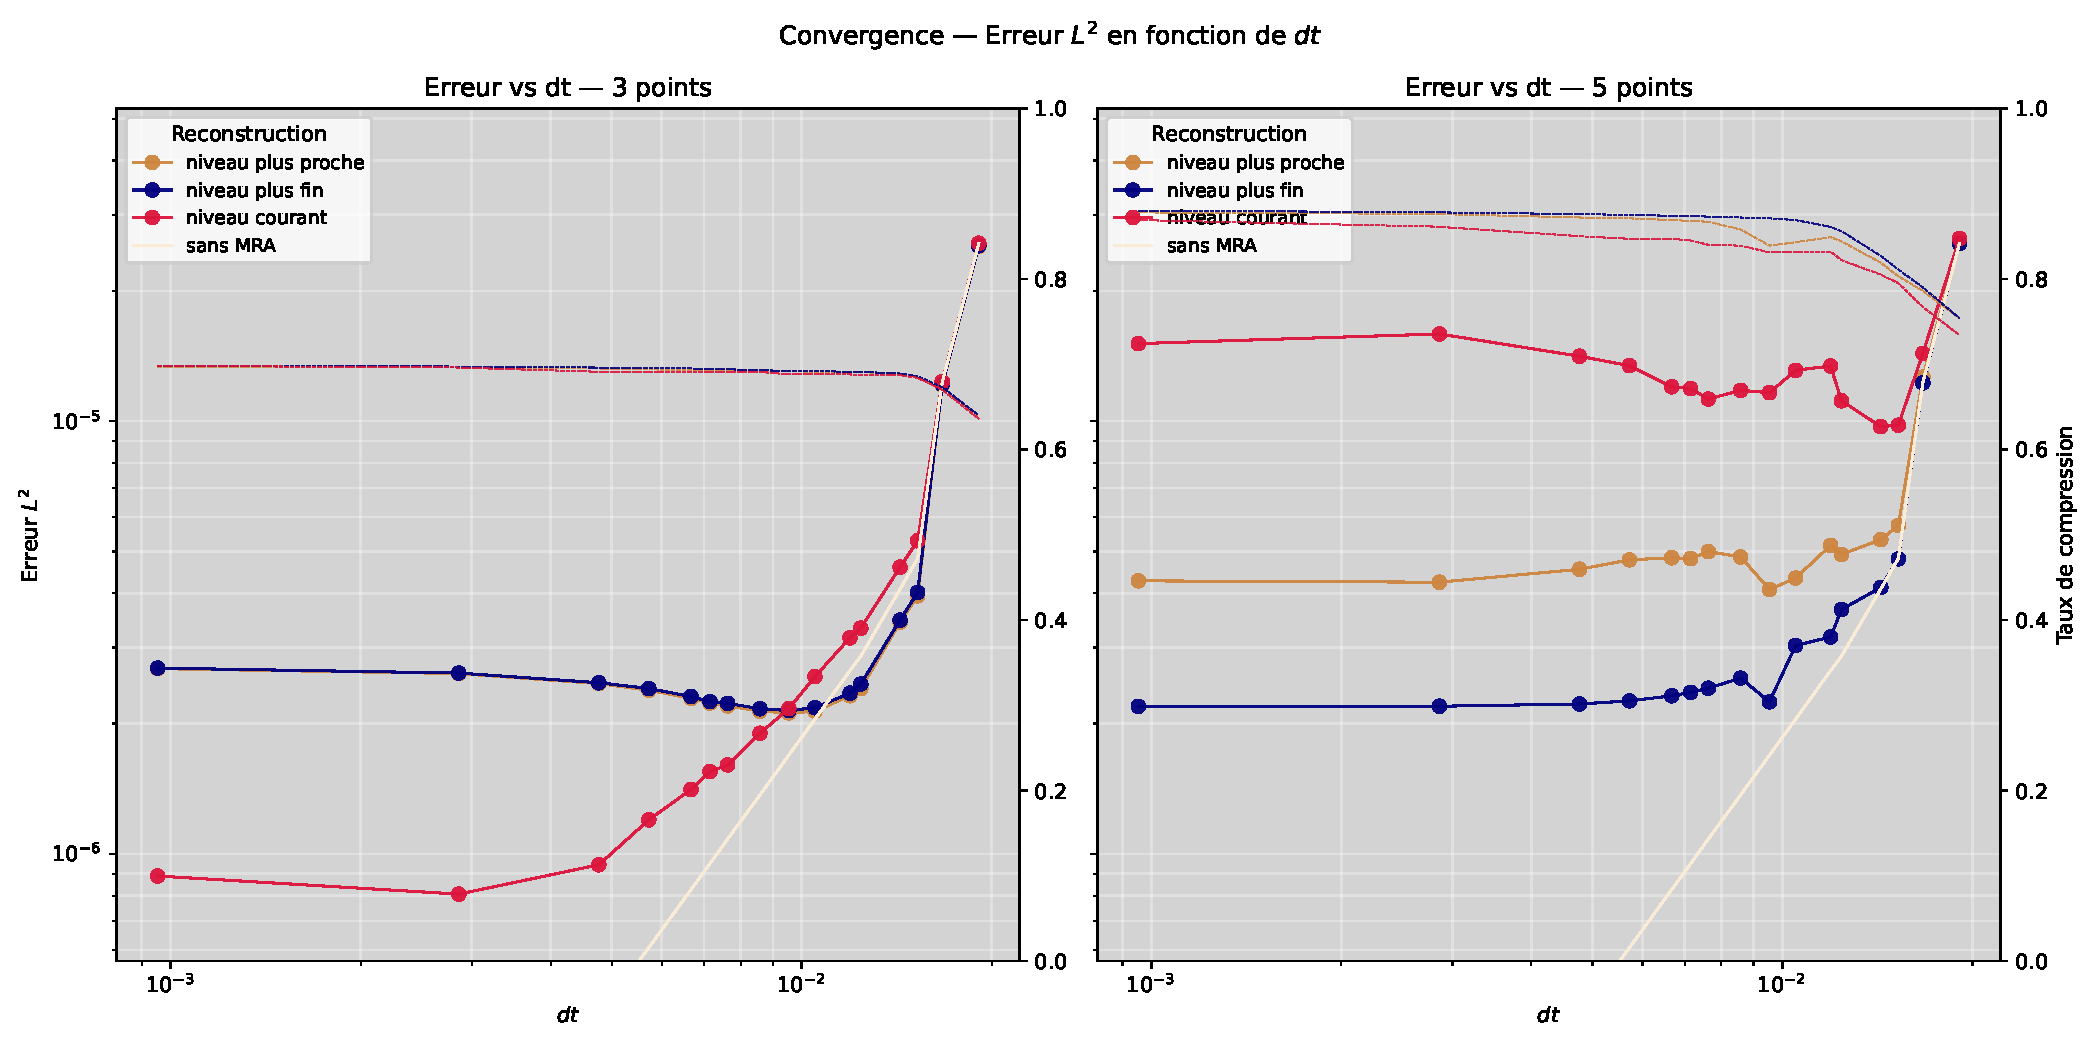
\includegraphics[width = \textwidth]{medias/3_/error_vs_dt_by_mlf.pdf}
\end{frame}
\begin{frame}{Complément}{Essais numériques - prédicteurs à 5 points}
    \begin{textblock*}{40pt}(0.05\paperwidth,0.88\paperheight)
\includegraphics[scale=.03]{medias/2_/1_/light_logo.png}\end{textblock*}
    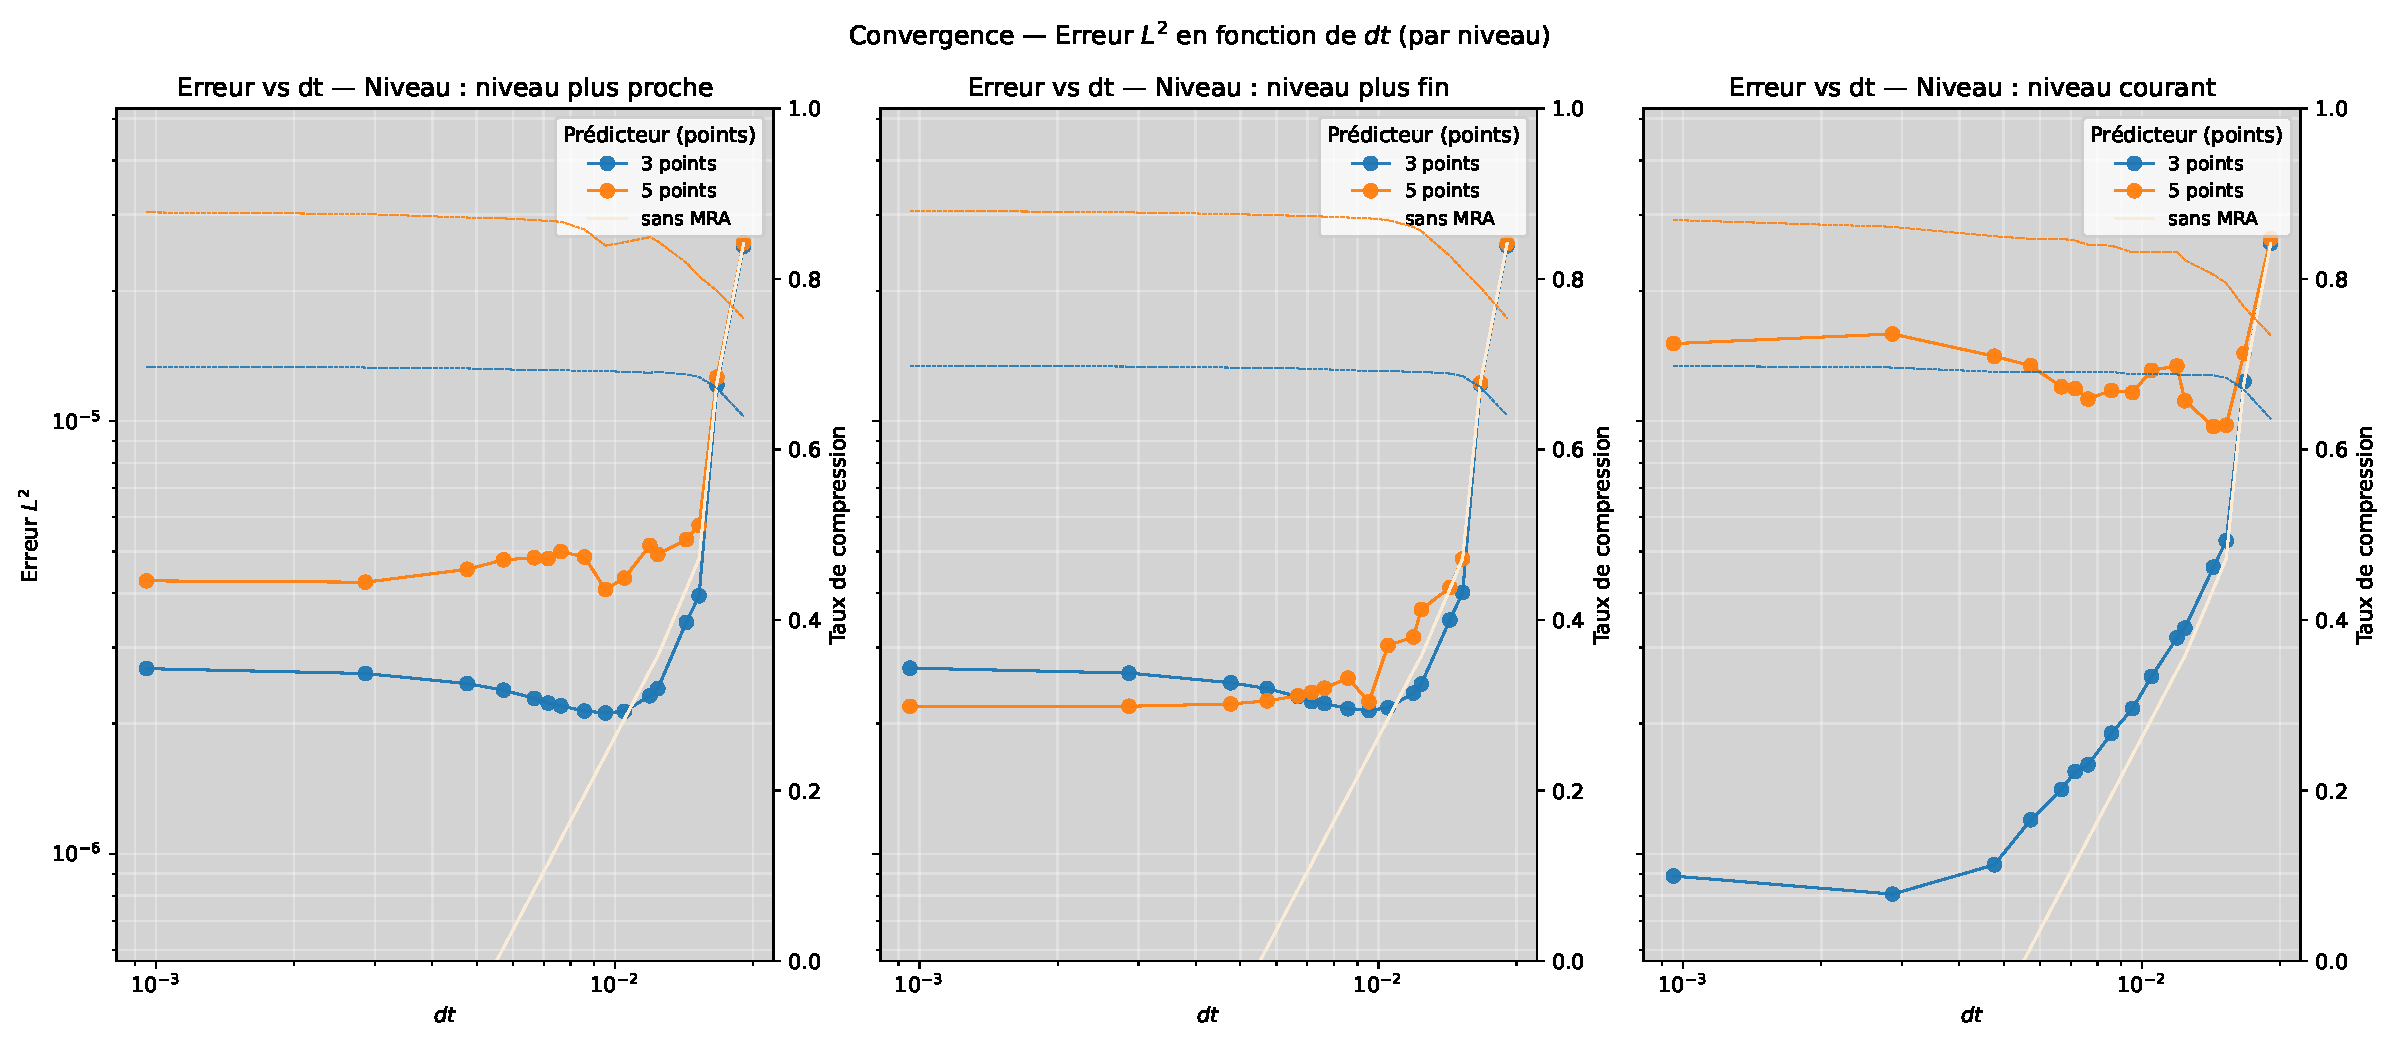
\includegraphics[width = \textwidth]{medias/3_/error_vs_dt_by_stencil_per_mlf.pdf}
\end{frame}
\section*{Compléments}
\paragraph*{Conclusion scientifique}
Ce stage pave le chemin vers une compréhension plus fine du comportement des schémas de multi-résolution adaptative appliqués aux problèmes de diffusion.
L’analyse théorique, fondée sur les équations équivalentes et les études de stabilité, a montré qu’un couplage peut apparaître entre les schémas d’intégration en temps et la MRA, réduisant l’ordre de convergence attendu.
Les expériences numériques ont révélé un phénomène surprenant : une reconstruction de flux plus précise ne garantit pas nécessairement une meilleure exactitude globale.
Si le lien entre théorie et expériences reste en partie à clarifier, la mise en évidence de ces phénomènes fournit une base solide et des pistes pour de futures investigations.
\paragraph*{Conclusion sur ma progression technique}
Sur le plan théorique, j’ai approfondi des domaines variés : méthodes de volumes finis \cite{LeVeque1990}, systèmes dynamiques et méthodes de Runge–Kutta additives \cite{HairerAndWanner1}, ainsi que la théorie des ondelettes, en résonance avec mes cours antérieurs.
Sur le plan pratique, je me suis familiarisé avec des outils puissants d’analyse (équations équivalentes, analyse de Von Neumann), avec des codes de recherche avancés tels que \texttt{Samurai}, et avec les exigences de la simulation numérique (estimation rigoureuse des erreurs, gestion de grilles de taille différente, instabilités).
J’ai aussi développé mes compétences de programmation scientifique en Python et en \texttt{C++}, ainsi que ma maîtrise de l’environnement Unix (terminal, git, bash).
Enfin, j’ai renforcé mes capacités de communication scientifique, en diffusant mes codes pour en favoriser la reproductibilité et en produisant des graphiques complexes mais lisibles, parfois interactifs.
\paragraph*{Conclusion personnelle}
Ce stage a confirmé mon appétence pour les mathématiques appliquées et le numérique, tout en réorientant mes aspirations vers des projets plus appliqués.
Je me projette désormais davantage dans des missions de R\&D où les méthodes mathématiques servent directement des objectifs économiques et technologiques concrets.
J’ai aussi mesuré la valeur du travail collectif : l’utilisation d’outils développés par l’équipe m’a permis de mener des expériences numériques ambitieuses, inaccessibles seul.
Cette expérience m’a montré combien la mutualisation des efforts, la réutilisation des outils et leur interopérabilité constituent des leviers essentiels pour gagner en efficacité et valoriser les savoir-faire de chacun.
% \paragraph*{Conclusion scientifique} Mon stage pave le chemin vers une compréhension fine du comportement des schéma de multi-résolution adaptative sur les problèmes de diffusion.
% Il ébauche une vision théorique grâce aux études de stabilité et aux équation équivalente auquel s'ajoute de nombreux résultats d'expériences numériques.
% L'étude théorique montre qu'un couplage peut apparaître entre les schémas de diffusion et la MRA, dégradant l'ordre de convergence. 
% Les expériences numériques ont révélé un phénomène surprenant: une meilleure reconstruction du flux de diffusion ne mène pas toujours à une meilleure précision du schéma.
% Le lien entre la vision théorique et les résultats expérimentaux est encore difficile à établir clairement. 
% Toutefois la connaissance de l'existence de ces phénomènes et les hypothèses proposées et testées aideront et orienterons de futures investigations.
% \paragraph*{Conclusion sur ma progression technique} Mon expérience au CMAP m'a beaucoup appris.\par
% \textbf{Sur le plan théorique} j'ai approfondi de nombreux champs scientifiques croisés dans mon parcours étudiant.
% L'étude dans les méthodes de volumes finis \cite{LeVeque1990} pour les lois de conservations prolonge les cours de physique de classe préparatoires ainsi que les cours de mécanique et de simulation numérique à l'\textsc{Ensta}.
% J'ai étudié également l'analyse et la simulation des systèmes dynamiques grâce à \cite{HairerAndWanner1} faisant écho au cours de système dynamique de l'\textsc{Ensta} et j'ai 
% approfondi mes connaissance sur les méthodes Runge et Kutta découverte dans mes cours de troisième année en étudiant les méthodes additives (ARK - ImEx). La théorie des ondelettes
% dans laquelle j'ai du me plonger pour comprendre la MRA a résonné avec mes précédentes expériences en traitement du signal.\par
% \textbf{Sur le plan pratique} je me suis familiarisé avec de puissants outils d'analyse numérique comme les équations équivalentes.
% J'ai également utilisé \texttt{Samurai}, un code de calcul de l'état de l'art et été confronté aux difficultés et subtilités de la simulation numérique (calcul rigoureux des erreurs, interpolation sur de grilles de taille différence...).
% Le stage fut également l'occasion de découvrir le calcul formel avec Sympy et l'opportunité d'améliorer mes compétences de programmation scientifique en Python et \texttt{C++} ainsi que d'avoir une expérience concrète avec l'environnement Unix: terminal, git, bash...
% J'ai étoffé mes capacités de communication scientifique, prenant l’habitude de rendre disponible en ligne mes codes pour favoriser la reproductibilité et
% proposant des graphiques complexes mais lisibles et parfois même interactifs. Enfin  j'ai du appliquer les compétences générales d'un ingénieur-chercheur en proposant des hypothèses et en les testant, ainsi qu'en
% étant critique et transparent sur mes méthodes, mes expériences et mes résultats.
% \paragraph*{Conclusion personnelle}
% Ce stage à confirmé mon appétence pour les mathématiques et le numérique tout en réorientant mes aspirations professionnelles vers projet plus appliquées.
% J'ai compris que je m’épanouirai plus sur des missions de R\&D où les mathématiques sont directement au service d'un projet économique concret.
% J'ai aussi pu mesurer la valeur du travail en équipe, du partage des compétences, des connaissances et des travaux de chacun. 
% Par exemple, le logiciel Samurai développé au CMAP m'a permis de réaliser rapidement beaucoup d'expériences numériques complexes. 
% De même les ressources fourni par Ponio, développé par Joselin Massot au CMAP m'ont permis d'intégrer vite et sans erreurs des méthodes d'intégrations en temps qui mataient pris plusieurs semaines à implémenter.
% Enfin et surtout, les expériences sur les questions numériques de Marc Massot, Christian Tenaud et Laurent Series m'ont orienté souvent vers les bonnes hypothèses et m'ont gradé des chemins sans Issus.
% Les gains offerts par la diversité de l'équipe et les effort pour la réutilisation des outils développés ainsi que leur interopérabilité m'a vraiment fais prendre conscience 
% des enjeux d'équipe, de gestion des talents, de valorisation des outils internes. 
\begin{frame}[allowframebreaks]{Références}
  \tiny % (optionnel : réduit la taille)
  \bibliographystyle{plain} % ou plain, ieee, etc.
  \bibliography{bibliographie}
\end{frame}

{
\usebackgroundtemplate{%
  \begin{tikzpicture}
    \node[opacity=0.15,inner sep=0pt] 
      {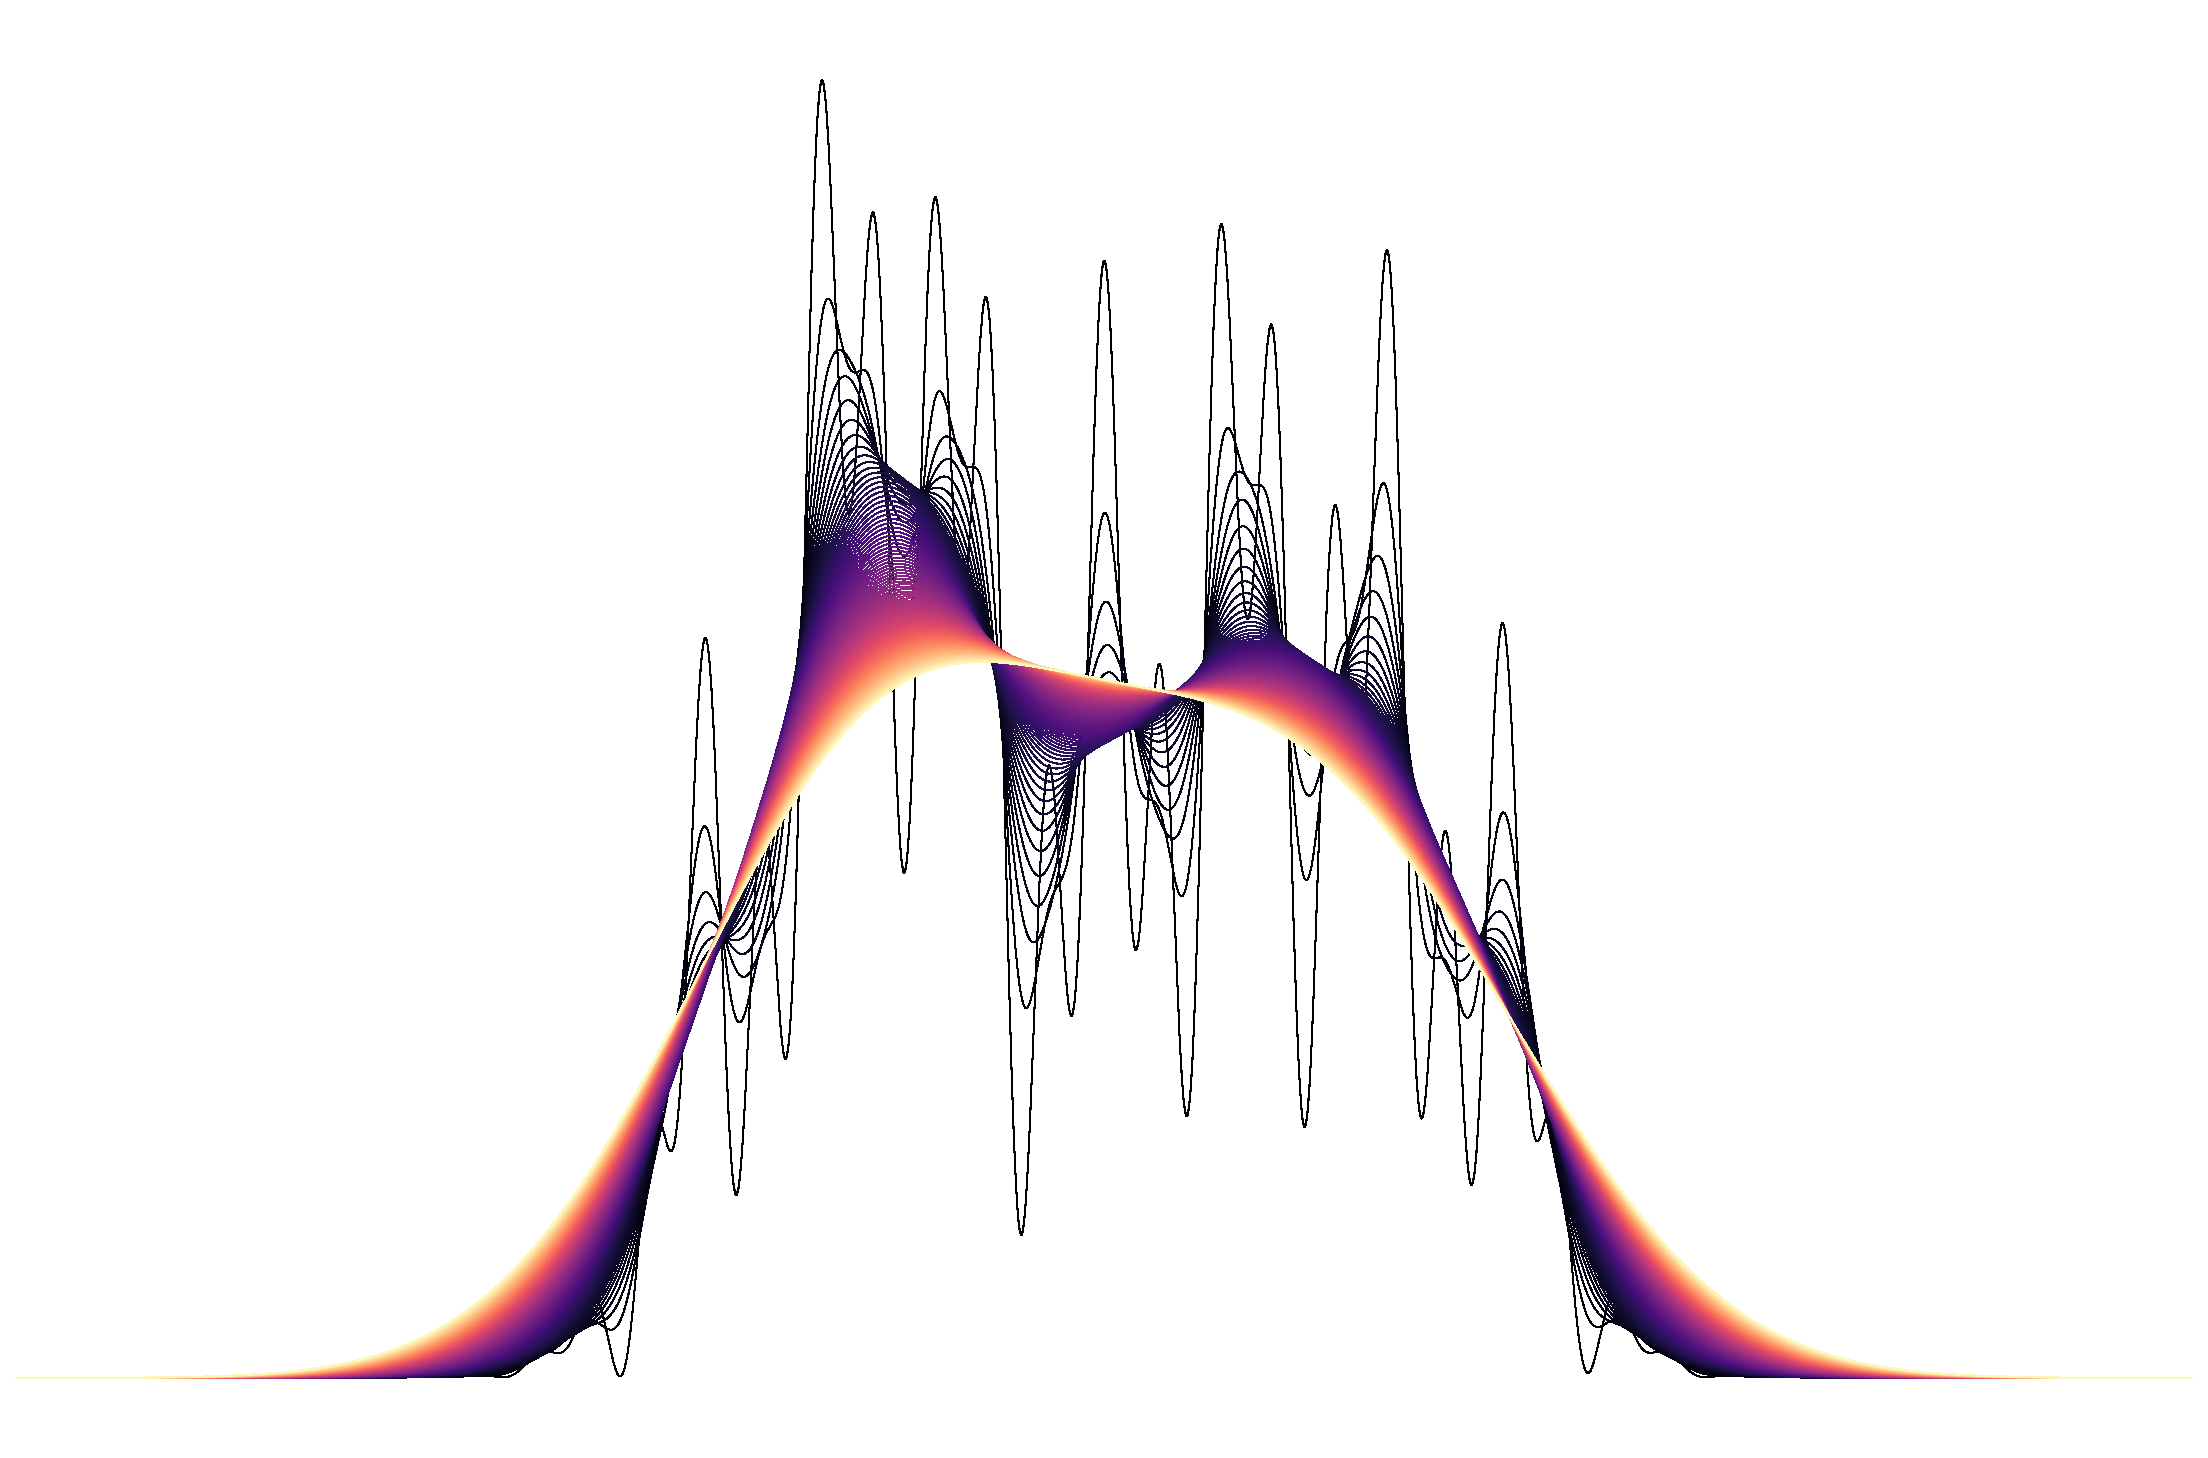
\includegraphics[width=\paperwidth,height=\paperheight]{medias/jolie_image_fin.pdf}};
  \end{tikzpicture}%
}
\begin{frame}[plain] % "plain" supprime header et footer
  \vspace{.8 \textheight} % pousse verticalement au centre
    \centering
\begin{tikzpicture}
  \node[opacity=0.3] {\LARGE\color{Primary}\textbf{MERCI !}};
\end{tikzpicture}

\end{frame}
}


\end{document}
